\documentclass[paper=a4,11pt,titlepage,twoside=true,headings=normal,numbers=noenddot,captions=tableabove,listof=totoc,index=totoc,bibliography=totoc]{scrreprt}
%\usepackage{amsmath} % abgesetzte Formeln zentriert in der Zeile
%\usepackage[fleqn,intlimits]{amsmath} % [fleqn] abgesetzte Formeln mit festem Abstand zum linken Rand
\usepackage[reqno,intlimits]{amsmath} % [reqno] um die gleichungsnummerierung rechts zu haben
% intlimits: Grenzen für Integrale unterhalb und oberhalb des Zeichens
\usepackage{amssymb}
\usepackage{array}
%\usepackage[ngerman]{babel}
%\usepackage[ngerman]{varioref}
\usepackage[english]{babel}
\usepackage[english]{varioref}
\usepackage[T1]{fontenc} 
\usepackage[utf8]{inputenc}
%---------------------------
\usepackage{booktabs}
\usepackage{calc}
\usepackage{cancel}
\usepackage[labelfont={footnotesize,sf,bf},textfont={footnotesize,sf}]{caption} %Format (Textgröße, Textform) für Bildtext 
%normalsize
%scriptsize
% sc --> smallcaps
% bf --> bold face
% sf --> sans serif
%\usepackage{cite} %inkompatibel mit biblatex
\usepackage[table]{xcolor}
%\usepackage{colortbl}
\usepackage[right]{eurosym}
%\usepackage{caption2} %nicht zusammen mit sidecap
%\usepackage{exscale}
\usepackage{ellipsis}
\usepackage{graphicx}
\usepackage{float}
%\usepackage{floatflt}
%----------------------------------------
\usepackage{gensymb} %-----------
%\usepackage{helvet}
\usepackage{csquotes}
\usepackage{listings}
\usepackage{longtable}
\usepackage{lastpage}  %----------
\usepackage{lscape}
\usepackage{lmodern}  %-- Silbentrennung
%\usepackage{mathpazo} % andere mathematische Symbol
\usepackage{makeidx}
%\usepackage{minitoc}
\usepackage{multirow}
\usepackage{multicol}
%\usepackage[intoc]{nomencl}   % zwei Spalten beim Formelzeichenverzeichnis
%\usepackage[german,intoc]{nomentbl} %vier Spalten bei Formelzeichenverzeichnis
\usepackage[english,intoc]{nomentbl} %vier Spalten bei Formelzeichenverzeichnis
\usepackage{nicefrac} %----
%\usepackage{picins} %----------
\usepackage{paralist} %--------
\usepackage{parallel}  %----------
\usepackage{pdfpages} %-------
% Define user colors using the RGB model
%\usepackage{colortbl}
%\definecolor{dunkelgrau}{rgb}{0.8,0.8,0.8}
%\definecolor{hellgrau}{rgb}{0.95,0.95,0.95}
%\usepackage{pgfplots}
\usepackage[figuresright]{rotating} 
\usepackage{scrlayer-scrpage}
%\usepackage[innercaption]{sidecap} %Beschriftung neben Bild, Tabelle, Mittelbach S333 %----------
%\usepackage{sistyle}
%\usepackage[locale=DE]{siunitx} %nicht zusammen mit sistyle %---------
\usepackage[locale=DE,per-mode=symbol,parse-numbers=false]{siunitx} %nicht zusammen mit sistyle %---------
\usepackage[font={scriptsize,sl},captionskip=3pt]{subfig} % für die Unterbilder %---------
\usepackage{shortvrb}
\usepackage{tablefootnote}
\usepackage{tabularx}
\usepackage{tabulary}
\usepackage{textcomp}
\usepackage{tocbasic}
%\usepackage{tikz}
\usepackage{times} 
\usepackage{units} %----------
\usepackage{url}
\usepackage{wrapfig} %----------
\usepackage{xr-hyper}
\usepackage{arydshln} %für \hdashline[5pt/2pt] % muss am Ende stehen, sonst gibt es Probleme mit xcolor
\usepackage{hyperref} % muss am Schluss stehen
\hypersetup{linkcolor={0 1 1}, linkbordercolor={1 1 1}, citebordercolor={1 1 1}} % setzt Linkboxen auf Farbe "`weiß"'
%\usepackage{bm}
%\usepackage[toc,symbols]{glossaries} %---------- muss nach hyperref stehen
\usepackage[nonumberlist, acronym, toc, section]{glossaries} % muss nach hypersetup stehen
%----------------
%\usepackage{romannum} % Seitenzahlen in römischen Ziffern
%\usepackage{adjustbox}
\usepackage{scrhack}
\usepackage[style=numeric, citestyle=numeric, backend=biber]{biblatex}
\usepackage[useregional]{datetime2}
\usepackage{cleveref} % löscht labels!!!!!!!!!! <--- warum? habs trotzdem eingefügt weil es die referencen nice macht ohne newcommands dafür zu brauchen. außerdem steht intellisense drauf ;)
\usepackage{isotope} % um chemische gleichungen hübscher darstellen zu können
\usepackage{framed} % rahmen um dinge malen können
\usepackage{svg} % um auch vektorgrafiken als bild einfügen zu können
\usepackage{adjustbox} % skaliert floats dynamischer (anti-over/underfull)
\usepackage[numbered]{bookmark} % platziert im pdf reader bei der kapitelübersicht die jeweiligen kapitelnummer vor die kapitelüberschriften
%-------------------------
 %\renewcommand{\captionlabelfont}{\sffamily} %für "Abbildung" und "Tabelle"
 %\renewcommand{\captionfont}{\sffamily\small} %für den Text der Bildunterschriften
%  \renewcommand{\captionlabelfont}{\sffamily} 
%  \renewcommand{\captionfont}{\sffamily} %\renewcommand{\normalfont}{\sffamily} %für die Überschriften
% Fettdruck der Bezeichnung Abbildung, Tabelle
%\renewcommand{\captionlabelfont}{\bfseries}
%---------------------------------------------
%------------------ Schrifttyp in der Kopf- und Fusszeilen
\setkomafont{pageheadfoot}{\footnotesize\sffamily}
%---------------------------------------------------
%Ändern der Abbildung- und Tabellenbezeichnung (Niedermair S.157)
%_____________________________________________
\addto\captionsngerman{\renewcommand\figurename{Abb.}}
\addto\captionsngerman{\renewcommand\tablename{Tab.}}
\renewcommand\listfigurename{Abbildungen}
%_______________________________
%Betrag eines Wertes
\newcommand{\abs}[1]{\lvert #1 \rvert} 
%---------------------------------------------
\newcommand{\absatz}[1]{\textbf{\textsc{#1}}} %siehe Mittelbach S. 876ff
%----------------------------
%\newcommand{\absatz}{\par \medskip}
%______________________________
%\newcommand{\anhang}[1]{Anhang \ref{#1}, Seite \pageref{#1}}
\newcommand{\anhang}[1]{Anhang \vref{#1}}
%________________________________
\newcommand{\aufgabe}{\stepcounter{plus} Aufgabe \arabic{plus}}
%______________________________________
%compactitem
\newcommand{\bci}{\begin{compactitem}}
\newcommand{\eci}{\end{compactitem}}
%______________________________________
%
\newcommand{\bi}{\begin{itemize}}
\newcommand{\ei}{\end{itemize}}
%______________________________________
%compactenumerate
\newcommand{\bce}{\begin{compactenum}}
\newcommand{\ece}{\end{compactenum}}
%_____________________________________
%begin equation
\newcommand{\be}{\begin{equation}}
\newcommand{\ee}{\end{equation}}
%_____________________________________
%begin equation ohne Formelnummer
\newcommand{\ben}{\begin{equation*}}
\newcommand{\een}{\end{equation*}}
%_____________________________________
%begin align ohne Formelnummer
\newcommand{\ban}{\begin{align*}}
\newcommand{\ean}{\end{align*}}
%_____________________________________
%begin align
\newcommand{\ba}{\begin{align} }
\newcommand{\ea}{\end{align}}
%_____________________________________
%minpage
\newcommand{\bmp}{\begin{minipage}[t]{.47\linewidth}}
\newcommand{\emp}{\end{minipage}}
%_____________________________
%  dB
\newcommand{\db}{dB}
%  dB(A)
\newcommand{\dba}{ dB(A) }
%  dB(A) für Satzende
\newcommand{\dbap}{ dB(A)}
%_________________________________
\newcommand{\bzw}{bzw.\,}
%_______________________________
\newcommand{\dif}{\mathrm{d}}
%________________________________
% neuer Zähler
\newcounter{plus}
\setcounter{plus}{0}
%______________________________
%Für das Formelverzeichnis _____________________ Formelverzeichis ____
% Befehl umbenennen in fz
\let\fz\nomenclature
% Deutsche Überschrift
\renewcommand{\nomname}{Formelzeichen}
% Punkte zw. Abkürzung und Erklärung
\setlength{\nomlabelwidth}{.20\hsize}
\renewcommand{\nomlabel}[1]{#1 \dotfill}
% Zeilenabstände verkleinern
\setlength{\nomitemsep}{-\parsep}
%_____________________________
\newcommand{\bild}[1]{Abb. \vref{#1}}
\newcommand{\sbild}[1]{siehe Abb. \vref{#1}}
\newcommand{\bilder}[2]{Abb. \vrefrange{#1}{#2}}
\newcommand{\bildseite}[1]{Abb. \vref{#1}} % erzeugt "`Abb. nn auf Seite nn
\newcommand{\tabelle}[1]{Tab. \vref{#1}}
\newcommand{\tabellenseite}[1]{Tab. \vref{#1}} % erzeugt "`Tab. nn auf Seite nn
% für \vref ist usepackage[german]{varioref} einzufügen
%_-------------------------------- Freiraum
\newcommand{\freiraum}[1]{\begin{figure}[H]\vspace{#1\textheight}\end{figure}}
%_____________________________
% Gleichung
\newcommand{\gl}[1]{Gl.\,(\ref{#1})}
\newcommand{\sgl}[1]{siehe Gl.\,(\ref{#1})}
\newcommand{\glbereich}[2]{Gl. \vrefrange[]{#1}{#2}}
%_____________________________
% Grad Celsius
\newcommand{\grad}{\,\degC}
\newcommand{\gradC}{\,\degree}
%______________________________________
% Großbuchstaben als Indizes kleiner schreiben; spezielle im Mathemodus
\newcommand{\klein}[1]{\scriptscriptstyle{#1}}% Fettdruck der Bezeichnung 
%______________________________
%% Kasten
\newcommand{\kasten}{\fbox{\rule{0.0pt}{10pt}{{ } } }}
%______________________________
%\newcommand{\kapitel}[1]{Kapitel \ref{#1}, Seite \pageref{#1}}
\newcommand{\kapitel}[1]{Kapitel \vref{#1}}
%_____________________________
%  LAeq für den äquivalenten Dauerschallpegel
\newcommand{\laeq}{ $L_{Aeq}$ }
%  LAeq für den äquivalenten Dauerschallpegel am Satzende
\newcommand{\laeqp}{ $L_{Aeq}$}
%_________________________________
%   Linie zeichnen
\newcommand{\linie}{\rule{0.5\textwidth}{0.1pt}}
%---------------------- LaTeX
\newcommand{\lt}{\LaTeX\,\,}
%----------------------------
\newcommand{\nl}{\newline}
%__________________________________
%  multicolumn für Tabellen
\newcommand{\mc}{\multicolumn}
%% \mc{1}{c}{Text}
%_________________________________
%    Parallel
\newcommand{\pl}[1]{\ParallelLText{#1}}
\newcommand{\pr}[1]{\ParallelRText{#1}}
\newcommand{\pp}{\ParallelPar}
%------------ rot unterstrichen
\newcommand{\rotunterstrichen}[1]{\textcolor{red}{\underline{\textcolor{black}{#1}}}}
%________________ Realteil
\newcommand{\real}[1]{\text{Re}\left\{#1\right\}}
%________________________________--
\newcommand{\seite}[1]{Seite \pageref{#1}}
\newcommand{\seiten}[2]{\vpagerefrange{#1}{#2}}
%----------------------------
%        TEXT Rot
\newcommand{\textrot}[1]{\textcolor{red}{#1}}
%______________________________
%Abkürzung für \multicolumn
\newcommand{\tab}[2]{\multicolumn{1}{#1}{#2}}
%_____________________________________
% doppelt unterstreichen
\newcommand{\unterstreichen}[1]{\underline{\underline{#1}}}
% einfach unterstreichen
\newcommand{\ul}[1]{\underline{#1}}
%______________________________
%kurze Verbatimausgabe
%\MakeShortVerb{\|} %mittelbach S.160 mit \usepackage{shortvrb}
%_______________________________________
% vspace
\newcommand{\vsf}{\vspace{5pt}}
%_________________________________
\newcommand{\zb}{z.B.\,}
\newcommand{\idr}{i.d.R.\,}
%_______________________________
% Zähler-einfach
\newcounter{req}
\newcommand{\zaehler}[1]{\refstepcounter{req}{#1} \thereq}
%% Beispielaufzählung \zaehler{Beispiel}\\
%_____________________________________
\setlength{\voffset}{-2.532 cm}
\setlength{\hoffset}{-1.57 cm}
% \setlength{\topmargin}{2.0 cm} \setlength{\topskip}{0.1 cm}
\setlength{\topmargin}{1.5 cm}
\setlength{\topskip}{0.1 cm}
\setlength{\evensidemargin}{1.5 cm}
\setlength{\oddsidemargin}{1.5 cm}
\setlength{\textwidth}{16.5 cm}
\setlength{\footskip}{40pt}
\setlength{\textheight}{24.5cm}
% \setlength{\textheight}{23.5 cm}
\setcounter{page}{1}
\setlength{\parindent}{0mm}
\setlength{\headsep}{20pt}
\setlength{\abovedisplayskip}{10pt}
\setlength{\belowdisplayskip}{10pt}
\setlength{\abovedisplayshortskip}{10pt}
\setlength{\belowdisplayshortskip}{10pt}
%----------------------------------------------------------------------
% Linien in der Kopf- und Fußzeile
%\renewcommand{\headrulewidth}{0.0pt}   %Linie in der Kopfzeile mit 0.0pt keine Linie
%%\renewcommand{\footrulewidth}{0.0pt}   %Linie in der Fußzeile mit 0.0 pt keine Linie
%\renewcommand{\headrulewidth}{0.2pt}   %Linie in der Kopfzeile mit 0.0pt keine Linie
%\renewcommand{\footrulewidth}{0.2pt}   %Linie in der Fußzeile mit 0.0 pt keine Linie
%------------------------------------------------------------------------
%\renewcommand{\normalfont}{\sffamily} %für die Überschriften
%\renewcommand{\chaptermark}[1]{\markboth{\chaptername\ \thechapter #1}{}}
%\renewcommand{\sectionmark}[1]{\markright{\thesection\ #1}}
% \rfoot{\leftmark\\\rightmark}

%Definitionen für Kopfzeile
% bei documentclass {report} hat der Eintrag für die [gerade Seite] keine Wirkung
%-------------------------------------------------------------
%%
%Einstellungen für Kopf- und Fusszeilen mit dem KOMA-Skript und \usepackage{scrpage2}
\pagestyle{scrheadings}
%\pagestyle{scrplain}
% le --> links, gerade Seite
% ce --> mittig, gerade Seite
% re --> rechts, gerade Seite
% lo --> links, ungerade Seite
% co --> mittig, ungerade Seite
% ro --> rechts, ungerade Seite
%---------------------------------------------
% Löschen aller Einträge
%\clearscrheadings
% \automark[section]{subsection}
% \pagemark --> Seitenzahl
% \automark --> Kapitelüberschriften
% \leftmark --> ??
% \rightmark --> ??
%::::::::::::::::::::::::::::::::::: Kopfzeile
% Kopfzeile gerade Seite
\automark[chapter]{chapter}
\lehead[]{\titelkopfzeilelinkseven}
\cehead[]{\titelkopfzeilemitteeven}
\rehead[]{\titelkopfzeilerechtseven}
% Kopfzeile ungerade Seite
\lohead[]{\titelkopfzeilelinksodd}
\cohead[]{\titelkopfzeilemitteodd}
\rohead[]{\titelkopfzeilerechtsodd}
% Linie in der Kopfzeile
%\setheadtopline{0.2pt} % obere Linie in der Kopfzeile; nur bei scrartcl
\setheadsepline{0.4pt} % untere Linie in der Kopfzeile; nur bei scrartcl
% Linie in der Fusszeile
%::::::::::::::::::::::::::::::::::: Fußzeile
% Fusszeile gerade Seite[plain-style]{scrheadings-style}
\lefoot[]{\titelfusszeilelinkseven} 
\cefoot[]{\titelfusszeilemitteeven}
\refoot[]{\titelfusszeilerechtseven}
% Fusszeile ungerade Seite
\lofoot[]{\titelfusszeilelinksodd}
\cofoot[]{\titelfusszeilemitteodd}
\rofoot[]{\titelfusszeilerechtsodd}
%\rofoot[\thepage ]{\thepage}
%\setfoottopline{0.2pt} % obere Linie in der Kopfzeile; nur bei scrartcl
\setfootsepline{0.4pt} % untere Linie in der Kopfzeile; nur bei scrartcl

% le --> links, gerade Seite
% ce --> mittig, gerade Seite
% re --> rechts, gerade Seite
% lo --> links, ungerade Seite
% co --> mittig, ungerade Seite
% ro --> rechts, ungerade Seite
% even --> gerade Seite
% odd --> ungerade Seite
%----------------------------------------- Kopfzeilentext
 \newcommand{\titelkopfzeilemitteeven}{}
 \newcommand{\titelkopfzeilemitteodd}{}
 \newcommand{\titelkopfzeilelinkseven}{Hochschule RheinMain}
 \newcommand{\titelkopfzeilelinksodd}{}
 \newcommand{\titelkopfzeilerechtseven}{}
 \newcommand{\titelkopfzeilerechtsodd}{Hochschule RheinMain}
 %----------------------------------------- Fußzeilentext
 \newcommand{\titelfusszeilemitteeven}{}
 \newcommand{\titelfusszeilemitteodd}{}
 \newcommand{\titelfusszeilerechtseven}{Studienbereich Angewandte Physik \& Medizintechnik}
 \newcommand{\titelfusszeilerechtsodd}{\thepage \hspace{0.5mm} von \pageref{LastPage}}
 \newcommand{\titelfusszeilelinkseven}{\thepage \hspace{0.5mm} von \pageref{LastPage}}
 \newcommand{\titelfusszeilelinksodd}{Studienbereich Angewandte Physik \& Medizintechnik}
\newcommand{\titelLV}{Physics Lab 3}
%---------------------------- VARIABLEN festlegen ------------------
%----------- Pro Versuch zu ändernde Angaben -----------------------
\newcommand{\versuch}{3} % Versuchsnummer einfügen
\newcommand{\untertitelb}{Torsional Pendulum} % Titel des Versuchs einfügen
\newcommand{\datumLV}{17.11.2020} % Datum einfügen
\newcommand{\deadline}{1.12.2020} % Abgabedatum ist der 1.12.2020
\newcommand{\dateLVa}{Dezember 15, 2020}
\newcommand{\dateLVb}{January 5, 2021}
%----------- TITEL
\newcommand{\untertitela}{Experiment P3-3}
% -------- Student 1
\newcommand{\nameA}{Hunter, Dennis}
% --------- Student 2
\newcommand{\nameB}{Kreß, Sebastian}
% --------- Student 3, falls vorhanden
\newcommand{\nameC}{Ünlü, Cihan}
%::::::::::::::::::::::::::::::::::
%\renewcommand\USenglishtoday
\DeclareNameAlias{author}{last-first}
\DeclareNameAlias{editor}{last-first}
\DeclareNameAlias{translator}{last-first}
\addbibresource{quellen.bib}
\begin{document}%\selectlanguage{USenglish}
%-----------------------------------------------------------------
\begin{titlepage} 
	\newcommand{\HRule}{\rule{\linewidth}{0.5mm}} 	
	\centering
	\textsc{\Large Hochschule RheinMain \\
		
\includegraphics[width=0.15\textwidth]{logo-hsrm}\\[1cm]}
%	\textsc{\Large Hochschule RheinMain}\\[1cm]
	\textsc{\LARGE \titelLV}\\[0.5cm]
		\HRule\\[0.4cm]
	{\huge\bfseries \untertitela}\\[0.4cm] % Title des Dokuments
	{\huge\bfseries \untertitelb}\\[0.4cm] % Title des Dokuments
		\HRule\\[1.5cm]
%-------------------
%\begin{flushleft}
	\begin{minipage}{0.4\textwidth}
%	\begin{flushleft}
%\centering
		\large
		\textit{\underline{Authors}}\\[0.5cm]
		\textsc{\nameA}\\[0.5cm]
		\textsc{\nameB}\\[0.5cm]
		\textsc{\nameC}\\[0.5cm]
		%\textsc{\nameC}\\[0.5cm] 
%	\end{flushleft}
\end{minipage}
%------------------------------------
\vfill\vfill\vfill 
%\textsc{\Large Fachbereich Ingenieurwissenschaften}\\[0.5cm]
\textsc{\Large Department of Engineering}\\[0.5cm]
%\textsc{\large Studienbereich Angewandte Physik \& Medizintechnik}\\[0.5cm]
\textsc{\large Applied Physics \& Medical Technology}\\[0.5cm]
\vfill
\begin{tabular}{ll}
	Date of experiment:\hspace{0.4cm} &{\large\dateLVa; \dateLVb}\\
	Date of submission:\hspace{0.4cm} &{\large\today} 
\end{tabular}
\end{titlepage}

%-----------------------------------------------------
\tableofcontents
\newpage
%--------------------
\chapter{Introduction}
%
\section{Terms and Definitions}
    \subsection*{Free Harmonic and Damped Oscillation}
        If a system capable of oscillation is deflected out of its equilibrium position and is experiencing a restoring force
        proportional to its deflection this system is called a \textit{harmonic oscillator}. If a dampening force such as friction
        is introduced, the system no longer oscillates freely but rather damped.\par
        Both, damped and harmonic oscillations are considered \textit{free} if there is no continuous, the oscillation driving
        stimulus present.
        %
    \subsection*{Natural Angular Frequency of a Harmonic Oscillation}
        %
        Depending on the very characteristics of the given system it will oscillate at a distinct frequency - the natural angular
        frequency \( \omega_0 \).
    \subsection*{Differential Equation of the Damped Harmonic Oscillation}
        \begin{equation}
            J \ddot{\varphi} = -D\varphi -\rho\dot{\varphi}+M\cos(\omega t) \footnote{\textcite{Eichler.2016}}
        \end{equation}
    \subsection*{Damping cases}
        Overdamped: The system returns to equilibrium without oscillating.\par
        Critically damped: The system returns to equilibrium as quickly as possible without oscillating.\par
        Underdamped: The system oscillates (at reduced frequency compared to the undamped case) with the amplitude gradually
        decreasing to zero.
    \subsection*{Rotational Inerta}
        A cylindrical rod has a rotational inertia about its center of: \(J_S = \frac{1}{12}ml^2\)
        %
    \subsection*{\textsc{Steiner}'s Theorem}
        \textsc{Steiner}'s Theorem: \(J = J_S + mr^2\)
        %
    \subsection*{Eddy Current Brake}
        The equivalent circuit of a conductor exposed to a changing magnetic field is composed of only a voltage source
        and a resistor. The voltage across this resistor is induced as of the law of electromagnetic induction: \(U_{ind} = -NA\frac{\partial B}{\partial t}\).
        The resulting current creates a magnetic field opposing the inducing field. If the change of the inducing magnetic
        field is due to a mechanical movement, the induced magnetic field will this movement as well.
        % Eddy currents are created when a conductor passes through a magnetic field, which creates opposing forces that spin
        % inside the conductor. According to Lenz’s law, an eddy current produces a magnetic field that is in opposition
        % to the magnetic field that produced it, and therefore eddy currents are an inverse response to the source magnetic field.
        %
    \subsection*{Constant Current Constant Voltage Operation of a PSU}
        As the name implies a power supply in CC/CV (\textbf{C}onstant \textbf{C}urrent/\textbf{C}onstant \textbf{V}oltage)
        operation mode keeps the output current and/or output voltage constant independently of the load applied.
        % In constant voltage mode, which is sometimes referred to as voltage-controlled mode, a power supply behaves like
        % a voltage source, holding the voltage across the output terminals constant while the current output varies,
        % depending on load conditions. Constant current mode is essentially the opposite of constant voltage mode. In
        % constant current mode, also known as current-controlled mode, the power supply behaves like a current source,
        % holding the current flowing through the output terminals constant while the output voltage varies depending on
        % load conditions.
        %
    \subsection*{Capacitance of a Parallel Plate Capacitor}\label{sec:capacitance of a parallel plate capacitor}
        The capacitance of a parallel plate capacitor is: \(C = \varepsilon_0 \varepsilon_r \cdot \frac{A}{d}\)
        %
    \subsection*{Time-Constant of an RC-Circuit}
        The time constant of an RC circuit: \(\tau = RC\)
    %
\section{Preparation}
%
    \subsection{Deriving the Equation for Damped Free Oscillation}\label{sec:preparation_task_1}
    %
        \begin{equation}
            \vec{M}_{ Inert } + \vec{M}_{ Frict } + \vec{ M}_{ Rest } = 0 \quad \Leftrightarrow \quad J \cdot \ddot\varphi(t) - k \cdot \dot\varphi(t) - D^* \cdot \varphi(t) = 0
        \end{equation}
        can be written as
        \begin{equation}
            \ddot\varphi(t) + 2 \delta \cdot \dot\varphi(t) + \omega_0^2 \cdot \varphi(t) = 0
            \label{eq:dampedOscillation}
        \end{equation}
        with
        \begin{equation}
            -\frac{k}{J} = 2\delta, \quad -\frac{D^*}{J} = \omega_0^2
            \label{eq:DEParameters}
        \end{equation}
        whereas \cref{eq:dampedOscillation} is a second degree harmonic differential equation.
        The chosen approach is:
        \begin{equation}
            \varphi(t) = \hat{\varphi} e^{\lambda t}, \quad \dot{\varphi}(t) = \lambda \hat{\varphi} e^{\lambda t}, \quad \ddot{\varphi}(t) = \lambda^2 \hat{\varphi} e^{\lambda t}
        \end{equation}
        Plugged into \cref{eq:dampedOscillation} gives
        \begin{align}
            \left(\lambda^2 + 2\delta \lambda + \omega_0^2\right) \hat{\varphi}e^{\lambda t} = 0 \nonumber \\
            \lambda_{1,2} = -\delta \pm \sqrt{\delta^2-\omega_0^2} \nonumber \\
        \end{align}
        Here two possible cases are to be distinguished:
        \begin{equation}
            \lambda_{1,2} =
            \begin{cases}
                    -\delta \pm i\omega_d \qquad \text{for} \qquad \delta^2 < \omega_0^2 \quad \text{(a)}\\
                    -\delta \pm \omega_d \qquad \text{for} \qquad \delta^2 \geq \omega_0^2 \quad \text{(b)}
            \end{cases}
        \end{equation}
        In \cref{eq:dampedOscillation}:
        \begin{equation}
            \varphi_1(t) = \varphi_1 e^{-\delta + i\omega_d t}, \quad \varphi_2(t) = \varphi_2 e^{-\delta - i\omega_d t}
        \end{equation}
        Linear combination of \( \varphi_1(t) \) and \( \varphi_2(t) \) lastly leads to
        \begin{equation}
            \varphi(t) = \varphi_1 e^{-\delta + i\omega_d t} + \varphi_2 e^{-\delta - i\omega_d t} = \hat{\varphi}e^{-\delta t} \cdot \cos{\left( \omega_d t + \varphi_0 \right)}
        \end{equation}
        %
    \subsection{Damping Cases}\label{sec:preparation_task_2}
    %
    \begin{figure}[H]
        \centering
        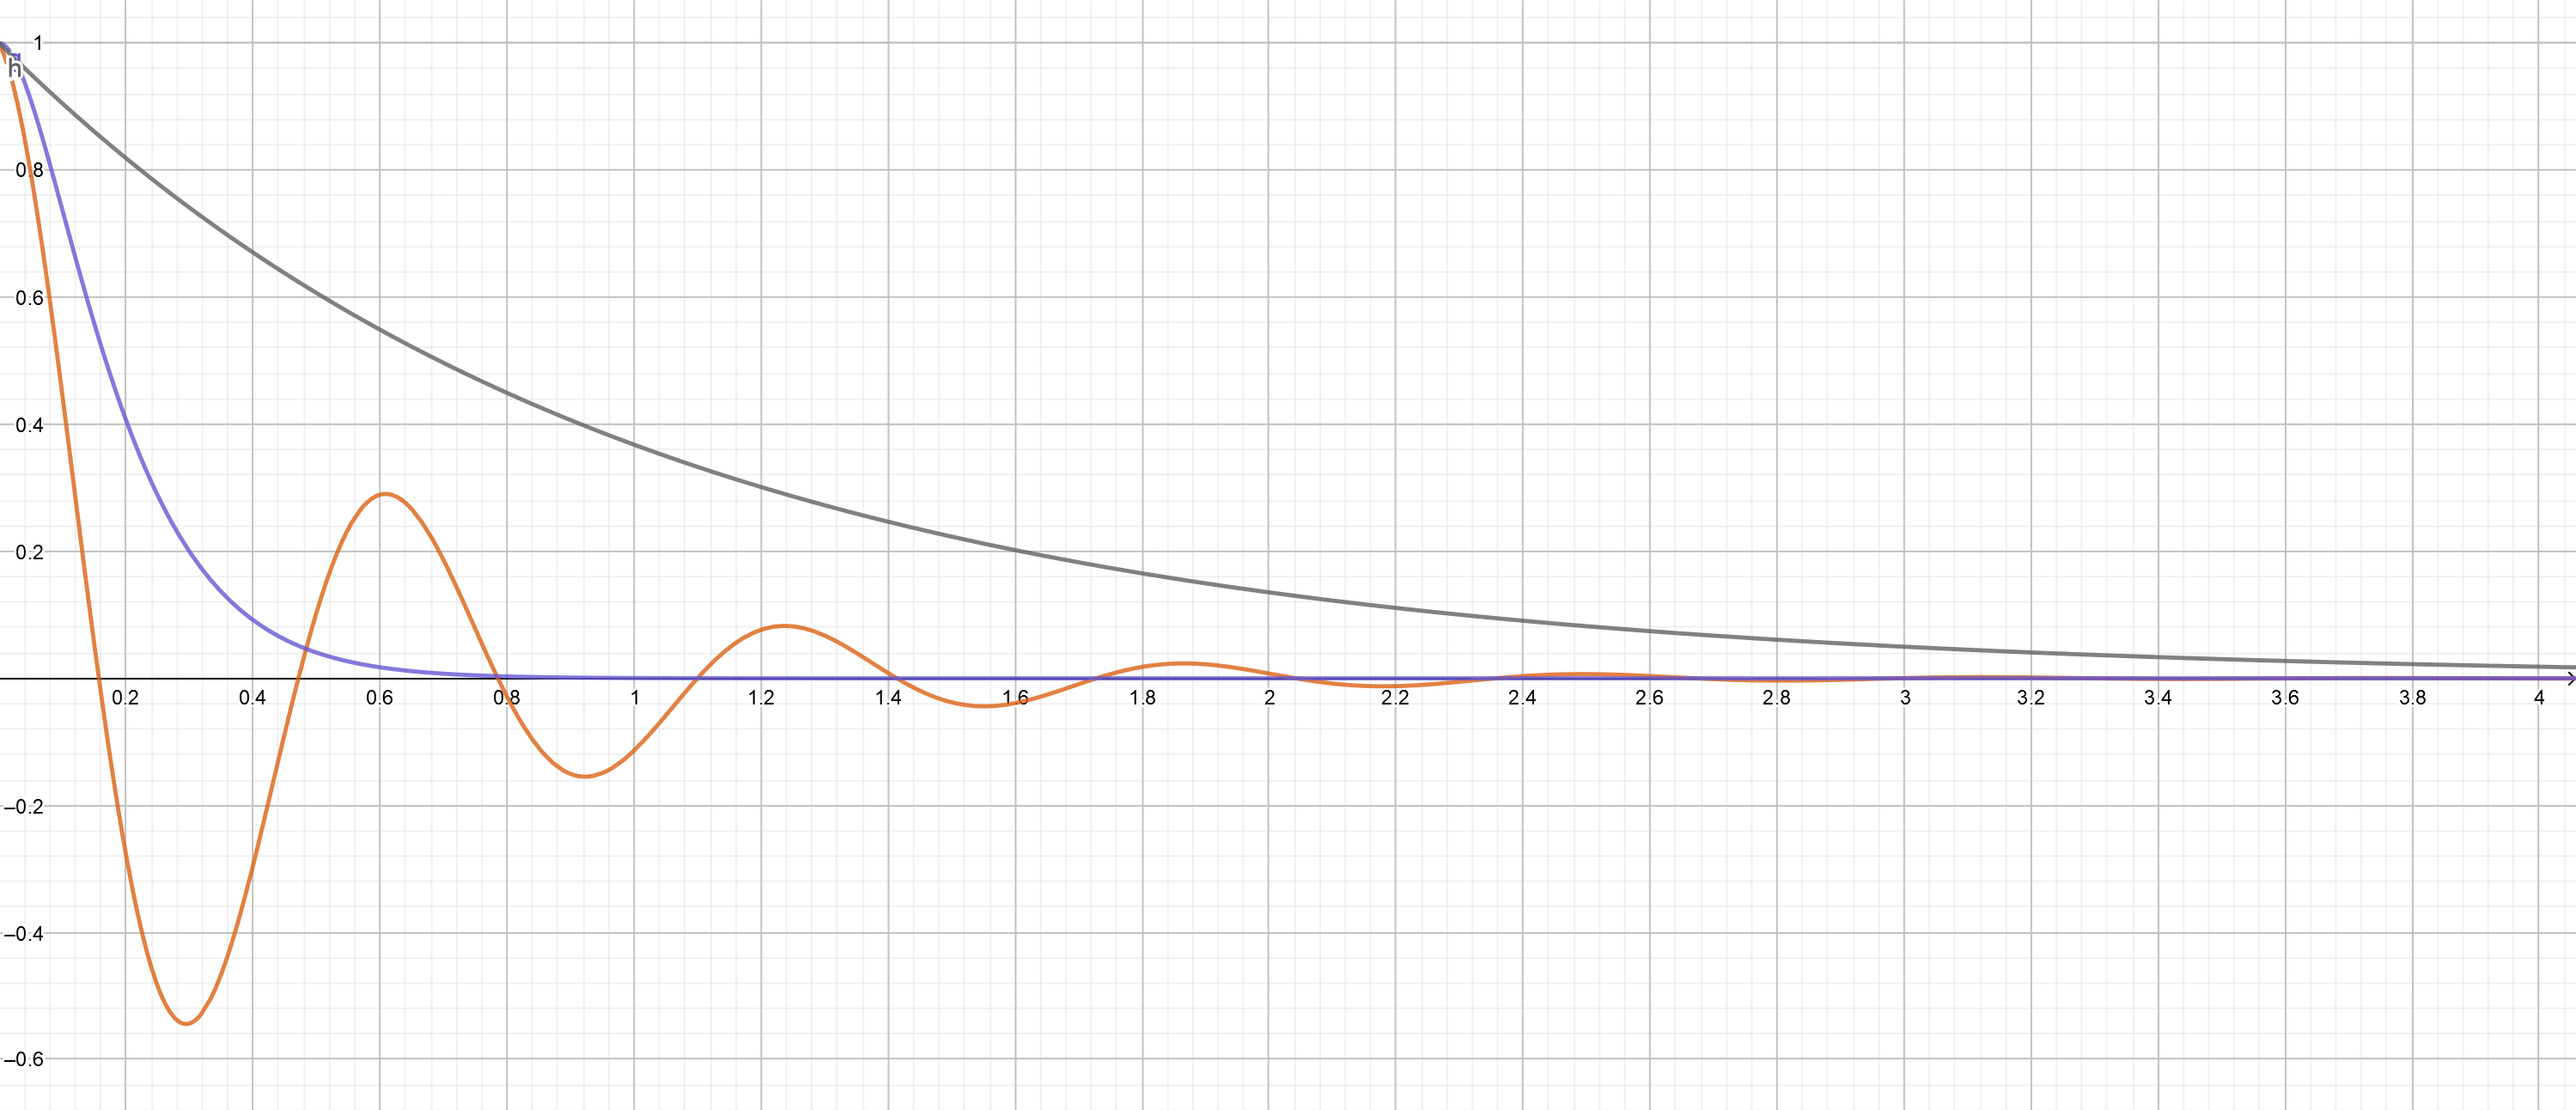
\includegraphics[width=.9\textwidth]{Preparation/damping_cases.png}
        \caption[Damping cases of a harmonic oscillation]{Plot of amplitude against time of a harmonic oscillation with
        parameterized damping coefficient. Orange: underdamped, Gray: overdamped, Blue: critically damped.}
        \label{fig:damping_cases_prepTask_2}
    \end{figure}
    %
    \subsection{Unknown Angular Inertia of the Pendulum}\label{sec:preparation_task_3}
    %
        The angular inertia of the pendulum \( J_P \) can be determined by adding a known angular inertia \( J_R \) of a cylindrical rod. As \cref{eq:DEParameters} delivers
        %
        \begin{equation}
            \omega_0=\sqrt{\frac{D^*}{J}}
        \end{equation}
        %
        and \( \omega=\frac{2\pi}{T} \), the following relation is given:
        %
        \begin{align}
            \omega_{0,P}=\sqrt{\frac{D^*}{J_P}}=\frac{2\pi}{T_P} \quad              &\Leftrightarrow \quad 2\pi=T_P\cdot\sqrt{\frac{D^*}{J_P}} \label{eq:omegaP} \\
            \omega_{0,P+R}=\sqrt{\frac{D^*}{J_P+J_R}}=\frac{2\pi}{T_{P+R}} \quad    &\Leftrightarrow \quad 2\pi=T_{P+R}\cdot\sqrt{\frac{D^*}{J_P+J_R}} \label{eq:omegaP+R}
        \end{align}
        %
        When \cref{eq:omegaP} and \cref{eq:omegaP+R} are equated:
        %
        \begin{align}
                                    &T_P\cdot\sqrt{\frac{D^*}{J_P}}=T_{P+R}\cdot\sqrt{\frac{D^*}{J_P+J_R}} \nonumber\\
            \Leftrightarrow \quad   &\left( \frac{T_{P+R}}{T_P} \right)^2 =\frac{J_P+J_R}{J_P}=1+\frac{J_R}{J_P} \nonumber\\
            \Leftrightarrow \quad   &\frac{J_R}{J_P}=\left( \frac{T_{P+R}}{T_P} \right)^2-1 \nonumber\\
            \Rightarrow \quad       &J_P=\frac{J_R}{\left( \frac{T_{P+R}}{T_P} \right)^2-1}
            \label{eq:inertia}
        \end{align}
        %
        The angular inertia of the pendulum can be calculated without knowing the torsion constant \( D^* \).
        %
    \subsection{Rotational Inertia of a Cylindrical Rod}\label{sec:preparation_task_4}
        %
        \begin{figure}[h]
            \centering
            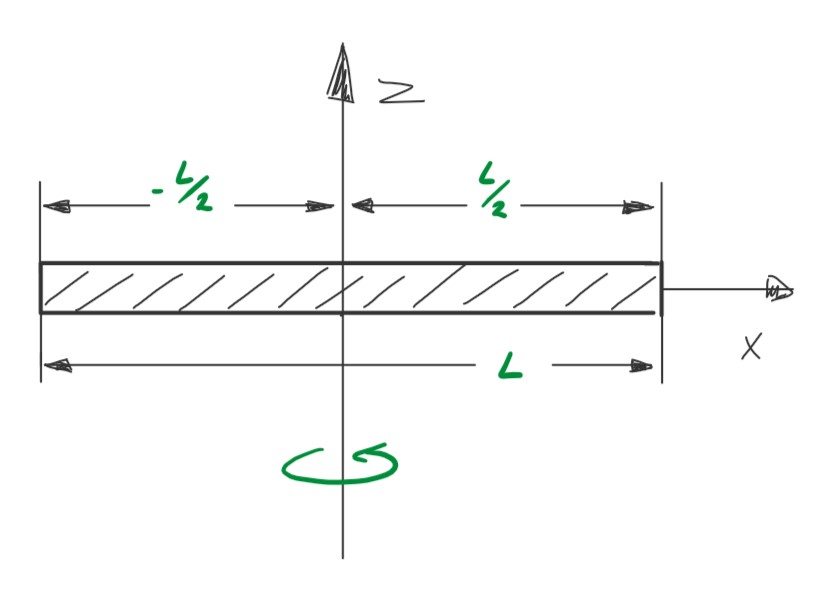
\includegraphics[width=.6\textwidth]{Preparation/rotating_rod.jpg}
            \caption[Rotating rod]{Scheme of a rod rotating orthogonally about its center axis.}
            \label{fig:rotationalIntertia_of_Cyl}
        \end{figure}
        %
        Inertia of a rotating dimensionless mass is proportional to the square of the distance to its rotational axis.
        As the mass of a cylindrical body is distributed over its volume, it is necessary to integrate over all \( dm  \) along
        the distance \( r \) from the center of rotation.
        \begin{equation}
            J_R = \int r^2 dm
            \label{eq:rotationalIntertia_of_Cyl}
        \end{equation}
        With
        \begin{equation}
            \rho = \frac{dm}{dx} = \frac{m}{L} \qquad \Leftrightarrow \qquad dm = \frac{m}{L} dx
        \end{equation}
        plugged into \cref{eq:rotationalIntertia_of_Cyl} with respect to the integration limits as of \cref{fig:rotationalIntertia_of_Cyl}
        gives
        \begin{equation}
            J_R = \int_{-\nicefrac{L}{2}}^{\nicefrac{L}{2}} \frac{m}{L} x^2 dx = \frac{1}{12}m L^2
            \label{eq:rotationalIntertia_of_Cyl alternate}
        \end{equation}
        %
    \subsection{Equations for the Sensor Capacitances}\label{sec:preparation_task_5}
        As described in \cref{sec:capacitance of a parallel plate capacitor}, the capacitance of a parallel plate capacitor
        is dependent on the overlapping area. Electrically, each vertical pair of capacitors are connected in parallel. They
        change there capacitance equally and in conjunction with the rotor rotating in any direction.\par
        % To derive:
        % \begin{align}
        %     C_1(\varphi) = \varepsilon_0 \frac{\pi D^2}{16 d} \left( 1 - \frac{2\varphi}{\pi} \right) \\
        %     \label{eq:capacitance 1 from tasks}
        %     C_2(\varphi) = \varepsilon_0 \frac{\pi D^2}{16 d} \left( 1 + \frac{2\varphi}{\pi} \right)
        %     \label{eq:capacitance 2 from tasks}
        % \end{align}
        % with
        % \begin{equation}
        %     A_{1,2}(\varphi) = \frac{1}{16}\pi D^2 \left( 1 \pm \frac{2\varphi}{\pi} \right)
        %     \label{eq:area from tasks}
        % \end{equation}
        %
        \begin{figure}[h]
            \centering
            \subfloat[Rotor at \( \varphi = \pm \frac{\pi}{2} \)\label{subfig:rotorAt pm halfPi}]{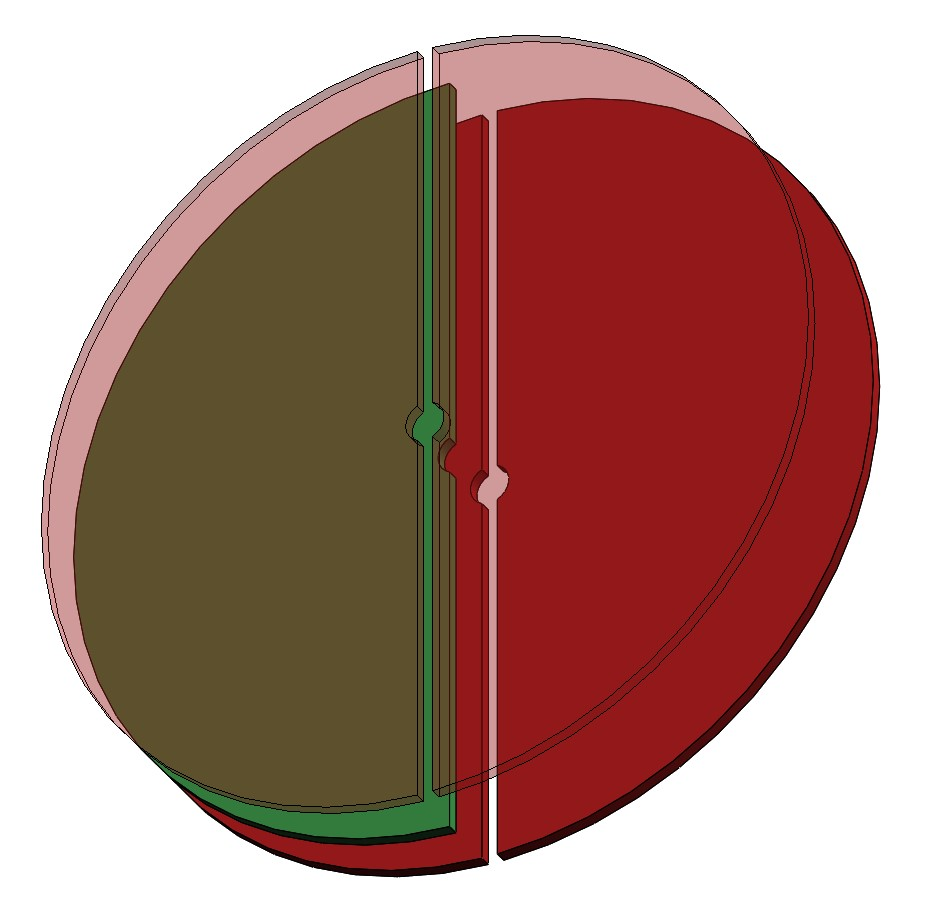
\includegraphics[width=.3\textwidth]{aufbau/statorRotorStator_pi.jpg}}
            \subfloat[Rotor at \( \varphi = 0 \)\label{subfig:rotorAt0}]{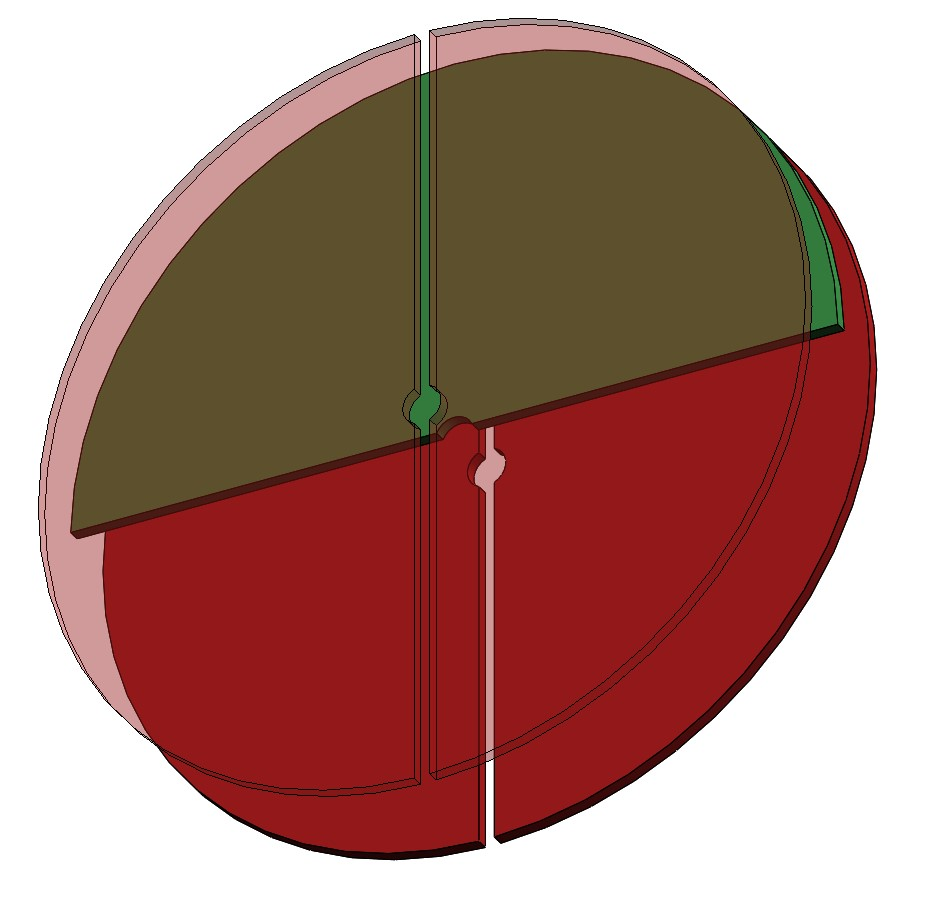
\includegraphics[width=.3\textwidth]{aufbau/statorRotorStator_0.5pi.jpg}}
            \subfloat[Rotor at \( \varphi = \mp \frac{\pi}{2} \)\label{subfig:rotorAt mp halfPi}]{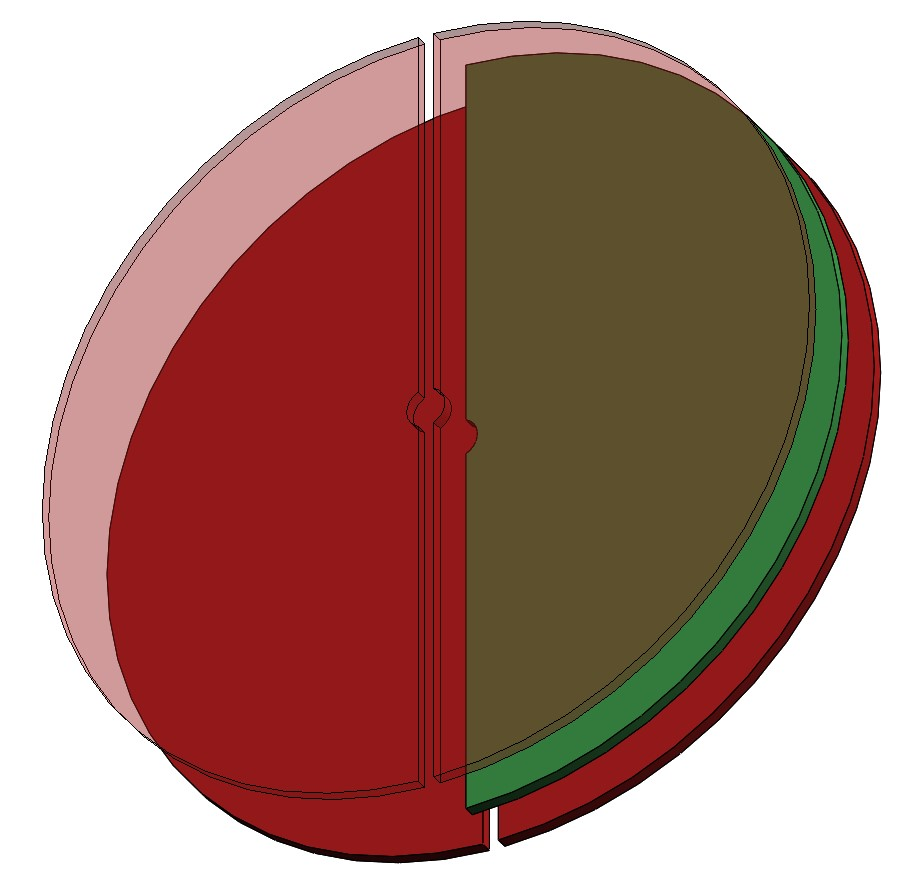
\includegraphics[width=.3\textwidth]{aufbau/statorRotorStator_0.jpg}}
            \caption[Schematic assembly of the angular sensor]{Schematic assembly of the angular sensor. The semi circular rotor plate (green) sandwiched between the two stators (red). The area of the rotor facing one of the vertical stator
            pairs varies with the angular displacement \( \varphi \)
            of the rotor.}
            \label{fig:rotorPositions}
        \end{figure}
        %
        Each of the vertically superimposed stator pairs together with the rotor plate form two capacitors connected in parallel
        with each capacitor having the same absolute value at any time. The total capacitance equates to
        \begin{equation}
            C_{1,2}(\varphi) = \varepsilon_0 \varepsilon_r \frac{A_{1,2}(\pm \varphi)}{d}
            \label{eq:angularCapacitance}
        \end{equation}
        Where \( A_{1,2}(\pm \varphi) \) can be expressed as
        \begin{align}
            A_{1,2}(\varphi)  &= \frac{1}{16}D^2 \left( \pi \pm 2\varphi \right) \nonumber \\
                        &= \frac{1}{16}D^2 \left( \frac{\pi^2}{\pi} \pm \frac{\pi}{\pi}2\varphi \right) \nonumber \\
                        &= \frac{1}{16} \pi D^2 \left( 1 \pm \frac{2\varphi}{\pi}\right)
            \label{eq:angularDependencyOfTheArea}
        \end{align}
        Say the zero-position is chosen such as each half of the rotor contributes to each of the stator pairs (see \cref{subfig:rotorAt0})
        \(A_1 = A_2\) applies. In any other case either \(A_1\) or \(A_2\) maximizes or minimizes respectively as shown in
        \cref{eq:rotation cases} (see \cref{subfig:rotorAt pm halfPi} and \cref{subfig:rotorAt mp halfPi} for reference).\par\medskip
        %
        Combining \cref{eq:angularCapacitance} and \cref{eq:angularDependencyOfTheArea} with \(\varepsilon_r = 1\) (air) gives
        %
        \begin{equation}
            C_{1,2} = \varepsilon_0 \frac{\pi D^2}{16d} \left( 1 \pm \frac{2\varphi}{\pi} \right) \quad \text{where} \quad \left(1 \pm \frac{2\varphi}{\pi} \right)
            \begin{cases}
                = 0 \quad \text{for} \quad \varphi = \mp \frac{\pi}{2} \nonumber \\
                = 1 \quad \text{for} \quad \varphi = 0 \nonumber \\
                = 2 \quad \text{for} \quad \varphi = \pm \frac{\pi}{2} \nonumber
            \end{cases}
            \label{eq:rotation cases}
        \end{equation}
        %
    \subsection{Time to Reach the Threshold Voltage}\label{sec:preparation_task_6}
        %
        The charging curve of a capacitor is given by \cref{eq:chargingCurve}.
        \begin{equation}
            U_C(t) = U_0 \left(1-exp\left(-\frac{t}{\tau}\right)\right)
            \label{eq:chargingCurve}
        \end{equation}
        Being interested at the time \( t_{th} \) it takes to reach a certain threshold voltage \( U_{th} \), \cref{eq:chargingCurve}
        can be transformed as follows:
        \begin{gather}
            1- \frac{U_{th}}{U_0} = exp\left(-\frac{t_{th}}{\tau}\right) \nonumber \\
            \Leftrightarrow \nonumber \\
            t_{th} = - \ln\left(1- \frac{U_{th}}{U_0}\right) \cdot \tau
            \label{eq:timeToThresholfVoltage}
        \end{gather}
        with the time constant \( \tau = R \cdot C \).
        %
    \subsection{Determining the Angular Deflection by the Difference of Timer Ticks}\label{sec:preparation_task_7}
        %
        The time to reach the threshold voltage as of \cref{eq:timeToThresholfVoltage} is captured independently due to
        each capacitor being connected to individual GPIOs.\par
        Since the charging curve of the capacitors differs in an anti-proportional manner when an angular deflection takes
        place the absolute value of the time difference gives the angle about zero while the sign gives the direction.
        Therefore, taken these considerations in account and merging \cref{eq:angularCapacitance} and \cref{eq:timeToThresholfVoltage}
        gives:
        \begin{align}
            \Delta t_{th}(\varphi)   &= t_{th,1} - t_{th,2} = -\ln\left( 1- \frac{U_{th}}{U_0} \right)R\left[ C_1(\varphi) - C_2(\varphi) \right] \nonumber \\
                            &= -\varepsilon_0 R \frac{\pi D^2}{16d} \ln\left( 1 - \frac{U_{th}}{U_0} \right) \left[ \left( 1 + \frac{2\varphi}{\pi} \right) - \left( 1 - \frac{2\varphi}{\pi} \right) \right] \nonumber \\
                            &= -\varepsilon_0 R \frac{4D^2}{16d} \ln\left( 1 - \frac{U_{th}}{U_0} \right) \cdot \varphi
            \label{eq:time_to_reach_thresholdVoltage}
        \end{align}
        Here \( \varepsilon_0 \), \( R \), \( D \), \( d \), \( U_{th} \) and \( U_0 \) remain constant and can be gathered as a proportionality
        factor. This reduces \cref{eq:time_to_reach_thresholdVoltage} to
        \begin{equation}
            \Delta t_{th}(\varphi) = \chi \cdot \varphi
            \label{eq:simplified_time_to_reach_thresholdVoltage}
        \end{equation}
        The \micro C checks the state of the input pin once every cycle. To take that into account the difference in threshold time
        \( \Delta t_{th} \) has to be divided by the cycle time \( \Delta t \) of the \micro C which gives the number of cycles it took for the
        input pins to switch state from low to high. If a change takes place at a non integer multiple of \( \Delta t \)
        the \micro C will register a transition on the subsequent cycle, thus, for the cycle count \( n \) applies \( n \in \mathbb{N} \).
        Furthermore, a non-integer value for \( n \) has to be rounded up to the next integer value.

        Mathematically the above considerations yield
        \begin{equation}
            n(\varphi) = \left\lceil \frac{\left\vert \Delta t_{th}(\varphi) \right\vert }{\Delta t} \right\rceil = \left\lceil \chi' \cdot \vert\varphi\vert \right\rceil \qquad \text{with} \qquad n(\varphi): n(\varphi) \in \mathbb{N}
            \label{eq:value_of_cycle_Count}
        \end{equation}
        which translates into the amount of deflection and
        \begin{equation}
            \frac{\vert n(\varphi)\vert}{n(\varphi)} = \pm 1
            \label{eq:sign_of_cycle_count}
        \end{equation}
        to distinguish between a CW/CCW rotation.
        %
    \subsection{Sensitivity of the Angular Sensor}\label{sec:preparation_task_8}
        %
        As seen in \cref{eq:simplified_time_to_reach_thresholdVoltage}, the tick rate relates linearly with the angular displacement \( \varphi \).
        Therefore, the maximum resolution of the angular sensor expressed as \textit{ticks per radiant} is \( \chi' \).
        \begin{equation}
            \frac{dn(\varphi)}{d\varphi} = \chi' \cdot \varphi \frac{d}{d\varphi} = \chi'
        \end{equation}
        \begin{figure}[H]
            \centering
            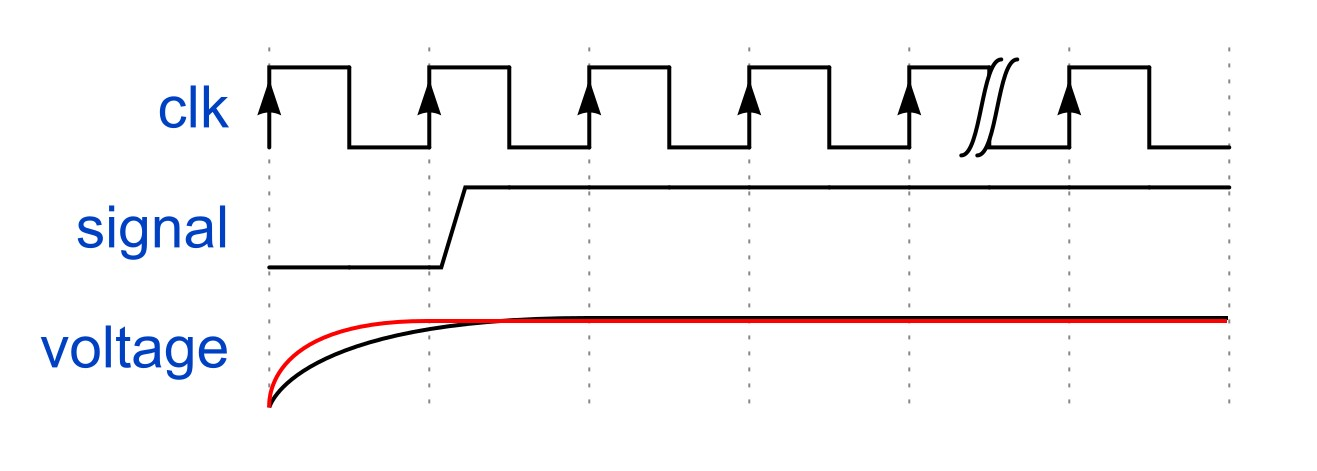
\includegraphics[width=.7\textwidth]{aufbau/clk_signal_timing_diagram.jpg}
            \caption[Timing diagram showing the signal transition]{Timing diagram showing the signal transition.}
            \label{fig:timing_diagram}
        \end{figure}
        The clock frequency of the \micro C is \( f = \SI{16}{MHz} \) which gives a cycle time of \( \Delta t = \SI{62.5}{ns} \).
        
        To ready the capacitors for the next charging cycle they need to be discharged as quick as possible. Considering
        that a time to discharge the capacitors \( < \Delta t \) makes no significant difference the unknown value \( R \)
        of the resistor can be approximated as
        \begin{gather}
            3\tau = \Delta t = 3RC \nonumber \\
            \Leftrightarrow \nonumber \\
            \frac{\Delta t}{3C_{max}} = R
            \label{eq:resistor_approximation}
        \end{gather}
        In the equation above the assumptions are made that a discharge rate of 95\% is sufficient and the circuit needs
        to be able to discharge the capacitor within the timeframe \( \Delta t \) while being at its maximum capacitance.
        Thus,
        \begin{align}
            C_{max} &= \varepsilon_0 \frac{\pi D^2}{8d} \nonumber \\
                    &= \SI{8,85\cdot10^{-12}}{\frac{\ampere\second}{\volt\metre}} \frac{\pi \cdot \SI{0.12^2}{m^2}}{8 \cdot \SI{0.01}{m}} \nonumber \\
                    &= \SI{5.01}{pF}
            \label{val:C_max}
        \end{align}
        in \cref{eq:resistor_approximation} gives a value for the resistance as
        \begin{equation}
            \frac{\SI{62.5}{ns}}{3 \cdot \SI{5.01}{pF}} \approx \SI{4160.9}{k\ohm}
        \end{equation}
        This lies between the two more common E-Series values of \(\SI{4.7}{k\ohm}\) and \(\SI{3.9}{k\ohm}\). For further calculations
        the latter is chosen as a higher resistance would increase the discharge time.\par\medskip
        Plugging in the given values of for \( \varepsilon_0, D, d, U_{th}, U_0 \) and the calculated values for \( \Delta t \text{ and } R \)
        equates \cref{eq:simplified_time_to_reach_thresholdVoltage} to
    
        \begin{align}
            \chi'   &= -\varepsilon_0 R \frac{4 D^2}{16d} \ln\left( 1 - \frac{U_{th}}{U_0} \right) \Delta t^{-1} \nonumber \\
                    &= -\SI{8.85 \cdot 10^{-12}}{\frac{As}{Vm}} \cdot \SI{3.9}{k\ohm} \cdot \frac{4 \cdot \SI{0.12^2}{\metre\squared}}{16 \cdot \SI{0.01}{\metre}} \ln\left( 1 - \frac{\SI{2.5}{\volt}}{\SI{5}{\volt}} \right) \cdot \frac{1}{\SI{62.5}{ns}} \nonumber \\
                    &\approx \SI{0.138}{\radian^{-1}}
                    \label{eq:est.sensitivity}
        \end{align}
        \nocite{Demtroder.2018.Experimentalphysik.1}\nocite{Eichler.2016}
\chapter{Set-Up of Experiment}
%
	The equipment and materials that are needed to perform the experiments are shown in \cref{fig:setup_total}. A detailed
	view of the angular sensor assembly is seen in \cref{fig:setup_detailed}.\par
	Using a desktop computer a serial connection via USB to the \micro C board is established. A serial monitor - \textsc{RealTerm} - is used to
	log the inbound stream send by the \micro C. The relevant settings are listed below:\par
	\begin{itemize}
		\item \SI{9600}{Baud}
		\item On the \texttt{Display} tab, \texttt{Ascii} and \texttt{new Line mode} need to be checked, \texttt{Direct capture}\par
		is un-checked.
		\item COM-Port as assigned by the OS.
	\end{itemize}
	%
	The data is now continuously sent by the \micro C. The data is displayed on the screen. A text file is created in
	which the data is written and saved. Two columns are displayed. The first column contains the time \(t\) in seconds, the
	second the number of timer ticks \(n\). The current source for the electromagnet is switched on.\par
	Now the setup is completed and the experiments can be started.
	%
	\begin{figure}[h]
		\centering
		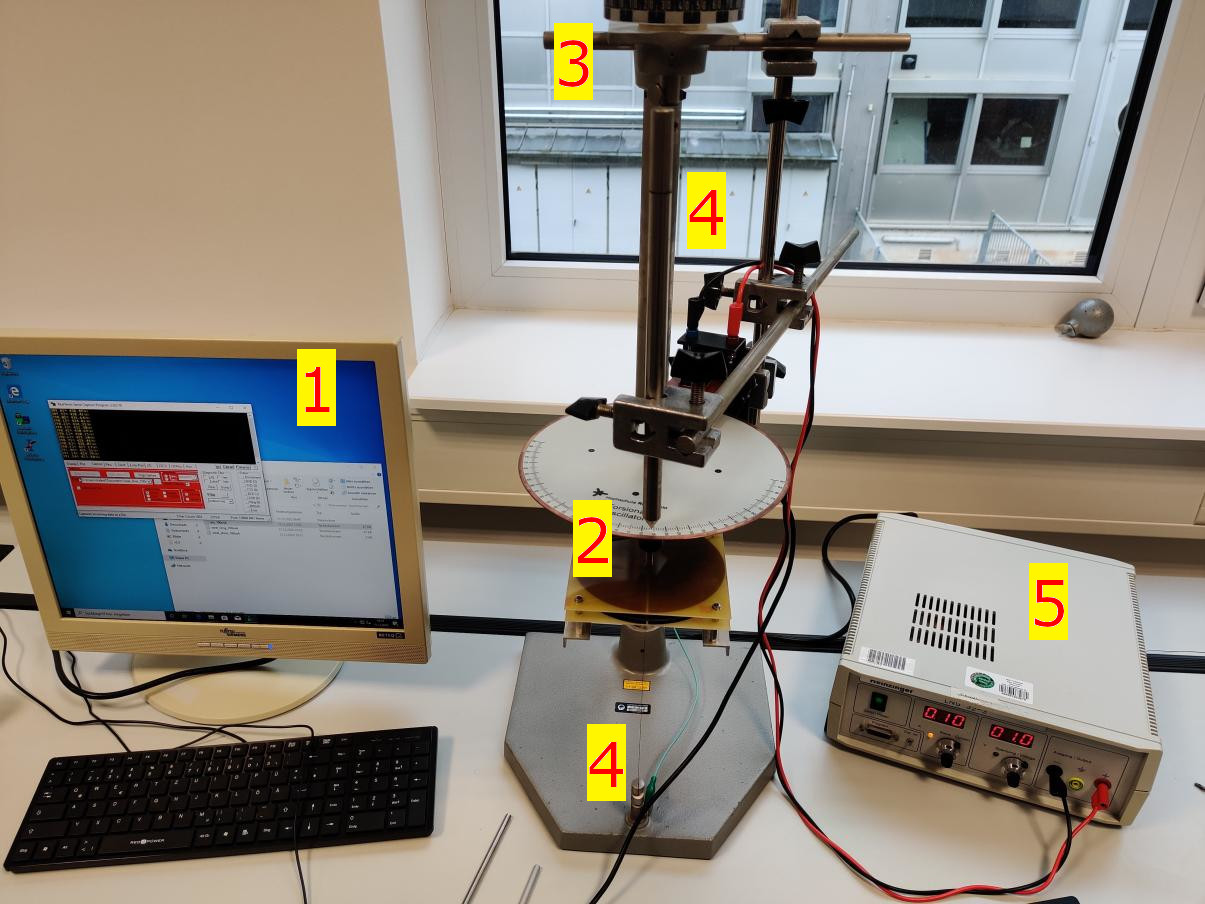
\includegraphics[width=.8\textwidth]{aufbau/setup_total_num.jpg}
		\caption[Equipment used.]{ Equipment and material required for the experiments. 1. Computer running \textsc{RealTerm}, 2. Angular sensor assembly,
		3. Zero adjustment, 4. Torsion wire, 5. PSU in constant current mode powering the eddy current brake.}
		\label{fig:setup_total}
	\end{figure}
	%
	\par
	%
	\begin{figure}[h]
		\centering
		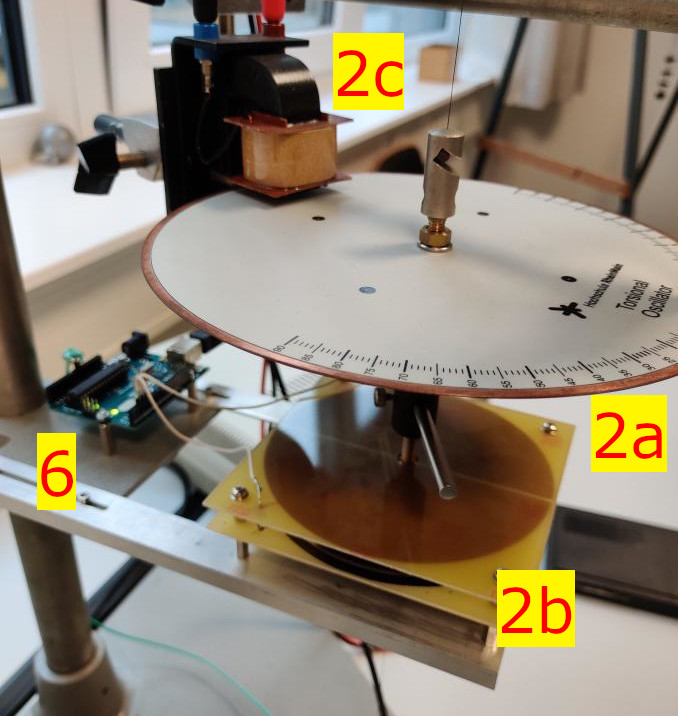
\includegraphics[width=.5\textwidth]{aufbau/setup_pendulum_side_num.jpg}
		\caption[Equipment in detail.]{ Detailed view of the angular sensor assembly. 2a: Copper plate with scale in degree, 2b: Capacitor plates, 2c: Eddy current brake,
		6: \micro C board.}
		\label{fig:setup_detailed}
	\end{figure}
	%
\input{chapters/4_durchführung}
\chapter{Evaluation}
%
\section{GMT Characteristics}
%
\subsection{Characteristic Values of the Oscilloscope}
%
The signal of the GMT can be seen on the oscilloscope screen. \cref{subfig:fig1pulsAmplitude} shows the base line \(U_{0}\) and
the amplitude \(\hat{U}\):
%
\begin{align}
U_{0}   &=  \SI{24}{mV} \pm \SI{40}{mV} \\
\hat{U} &=  \SI{1,56}{V} \pm \SI{0,04}{V}
\end{align}
%
Further there can be read off the fall time \(t_{f}\) (\cref{subfig:fig2fallTime}), rise time \(t_{r}\) (\cref{subfig:fig3riseTime}), the pulse width \(t_{p}\)
(\cref{subfig:fig4pulseWidth}) and recovery time \(t_{r}\) (\cref{subfig:fig5recoveryTime}):
\begin{align}
t_{f}   &=  \SI{56}{\micro s} \pm \SI{20}{\micro s} \\
t_{r}   &=  \SI{228}{\micro s} \pm \SI{20}{\micro s} \\
t_{p}   &=  \SI{108}{\micro s} \pm \SI{20}{\micro s} \\
t_{re}  &=  \SI{288}{\micro s} \pm \SI{20}{\micro s}
\end{align}
%
\subsection{Characteristic Curve of the GMT}
%
After determining the starting voltage \(U_{start}\) to \(U_{start}=\SI{328}{V}\), the characteristic curve has been
recorded. The calculated mean value
of the count rate has been plotted versus the mean voltage by \textsc{SciDAVis}:\par
\begin{figure}[H]
 \centering
 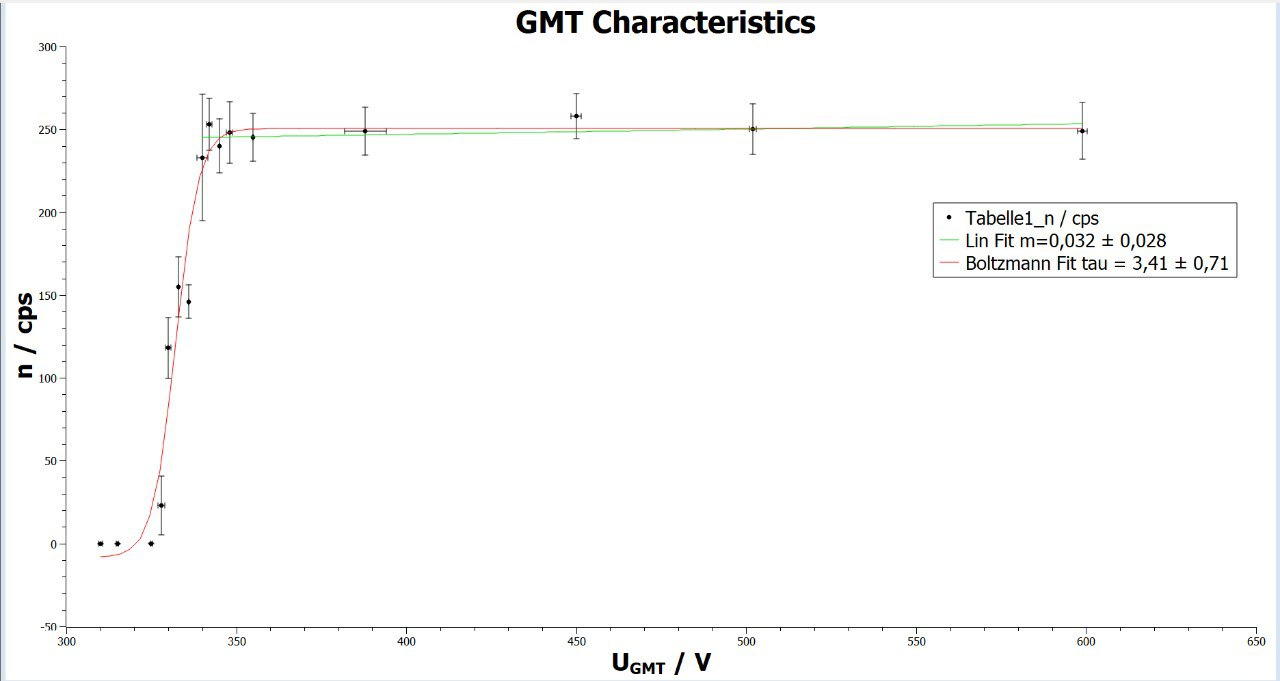
\includegraphics[width=.9\textwidth]{scidavis/Fig.6_GMT-characteristics.jpg}
 \caption[GMT characteristic]{Plot characterising the operating GMT.}
 \label{fig:gmtCharacteristics}
\end{figure}
The relative slope in the plateau area is determined to \(m=(3,2 \pm 2,8) \frac{\%}{\SI{100}{V}}\).\par
The optimum working voltage \(U_{opt}\) is determined to \(U_{opt}=\SI{500}{V}\), since the maximum possible adjustable
voltage of \(U_{GMT}=\SI{600}{V}\) is still in the plateau area, which starts at \(U_{GMT}=\SI{340}{V}\).
%
\section{Angular Dependency of the Count Rate}
To examine the angular dependency the count rate was measured at the optimum working voltage of
\(U_{opt}=\SI{500}{V}\) and the mean values of the 12 count rates of each angle were calculated. After that, the count
rate versus angle was given as:\par
\begin{figure}[H]
 \centering
 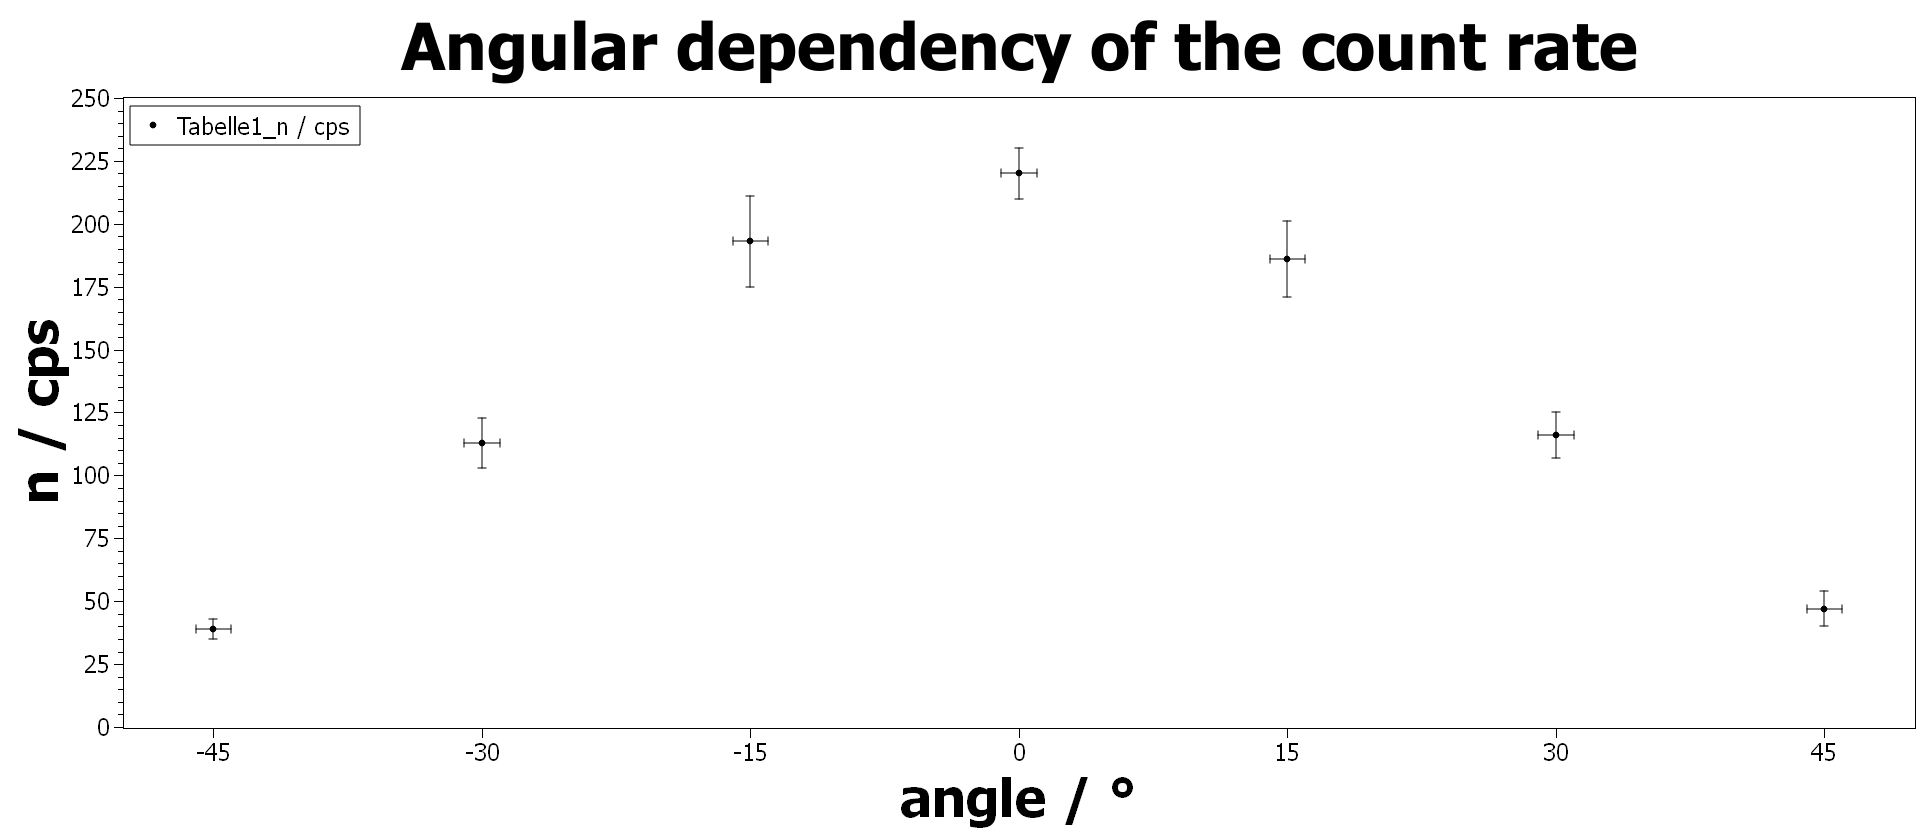
\includegraphics[width=.8\textwidth]{scidavis/Fig.7_Angular dependency of the count rate.jpg}
 \caption[Angular dependency of cps]{Angular dependency of the measured count rate.}
 \label{fig:angularDepCPS}
\end{figure}
%
\section{Absorption Characteristics of Materials}
%
For investigating the absorption characteristics of materials, the means of the count rates at
\(U_{opt}=\SI{500}{V}\) for different materials were determined:
%
\begin{align}
&\text{no absorbing material: }  &&n = \SI{221}{cps} \pm \SI{11}{cps}\\
&\text{Aluminum (Al): }          &&n = \SI{10}{cps} \pm \SI{4}{cps}\\
&\text{Lead (Pb): }              &&n = \SI{7}{cps} \pm \SI{2}{cps}\\
&\text{Tin (Sn): }               &&n = \SI{6}{cps} \pm \SI{2}{cps}\\
&\text{Acrylic glass: }          &&n = \SI{26}{cps} \pm \SI{5}{cps}\\
&\text{Cardboard: }              &&n = \SI{104}{cps} \pm \SI{8}{cps}
\end{align}
%
The explanation for the different absorption of the different materials is the mass attenuation coefficient of the
different materials. The mass attenuation coefficient is dependent on the material density and the attenuation
coefficient. Since the attenuation coefficient depends on the atomic number, the size of the atom does
matter. The reason why there is happening an attenuation is because of the \(\alpha\)-, \(\beta\)- and \(\gamma\)-rays are
interacting with the material atoms. While the \(\alpha\)- and \(\beta\)-rays have a strong interaction with the material,
\(\gamma\)-rays have better penetration due to less likeliness to interact. The smaller the half-value layer of a
material the weaker the penetration. With lead (\isotope[82]{Pb}) and Tin (\isotope[50]{Sn}) and presumably Aluminum
(\isotope[13]{Al}) as well almost all rays are absorbed (dependent on the ray energy). Acrylic glass can probably be
traversed by the \(\gamma\)-rays. Due to there size already a thin sheet of cardboard is sufficient to absorbed
\(\alpha\)-ray particles almost entirely.
%
\section{Counting Statistics}
%
After 90 measurements we obtained the following statistical values for mean \( \bar{n} \), variance \( \sigma^{2} \) and standard deviation
\( \sigma \):
%
\begin{align}
\bar{n}     &=  \SI{4327}{cps} \\
\sigma^{2}  &=  \SI{4168}{(cps)^{2}} \\
\sigma      &=  \SI{65}{cps}
\end{align}
The measurement series results in a scatter plot as shown in \cref{fig:countingStatistics}.
\begin{figure}[H]
 \centering
 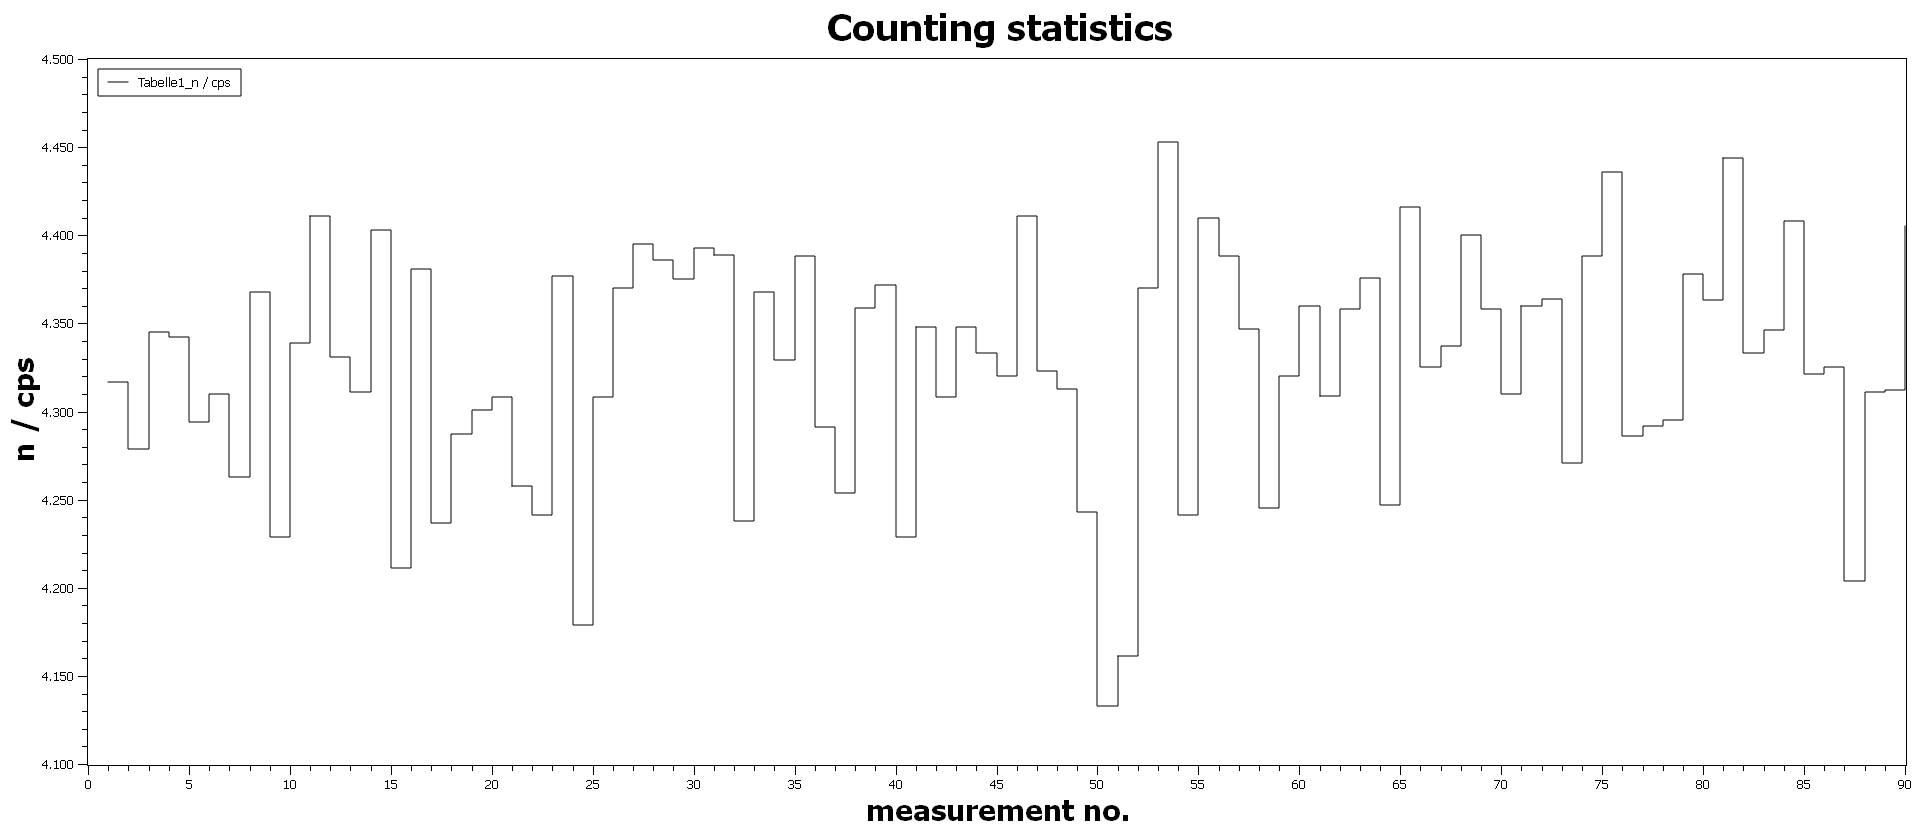
\includegraphics[width=.8\textwidth]{scidavis/Fig.8_Counting statistics.jpg}
 \caption[Counting statistics]{Counting statistics.}
 \label{fig:countingStatistics}
\end{figure}
with the associated histogram of distribution as seen in \cref{fig:countStatsHistogram}:
\begin{figure}[H]
 \centering
 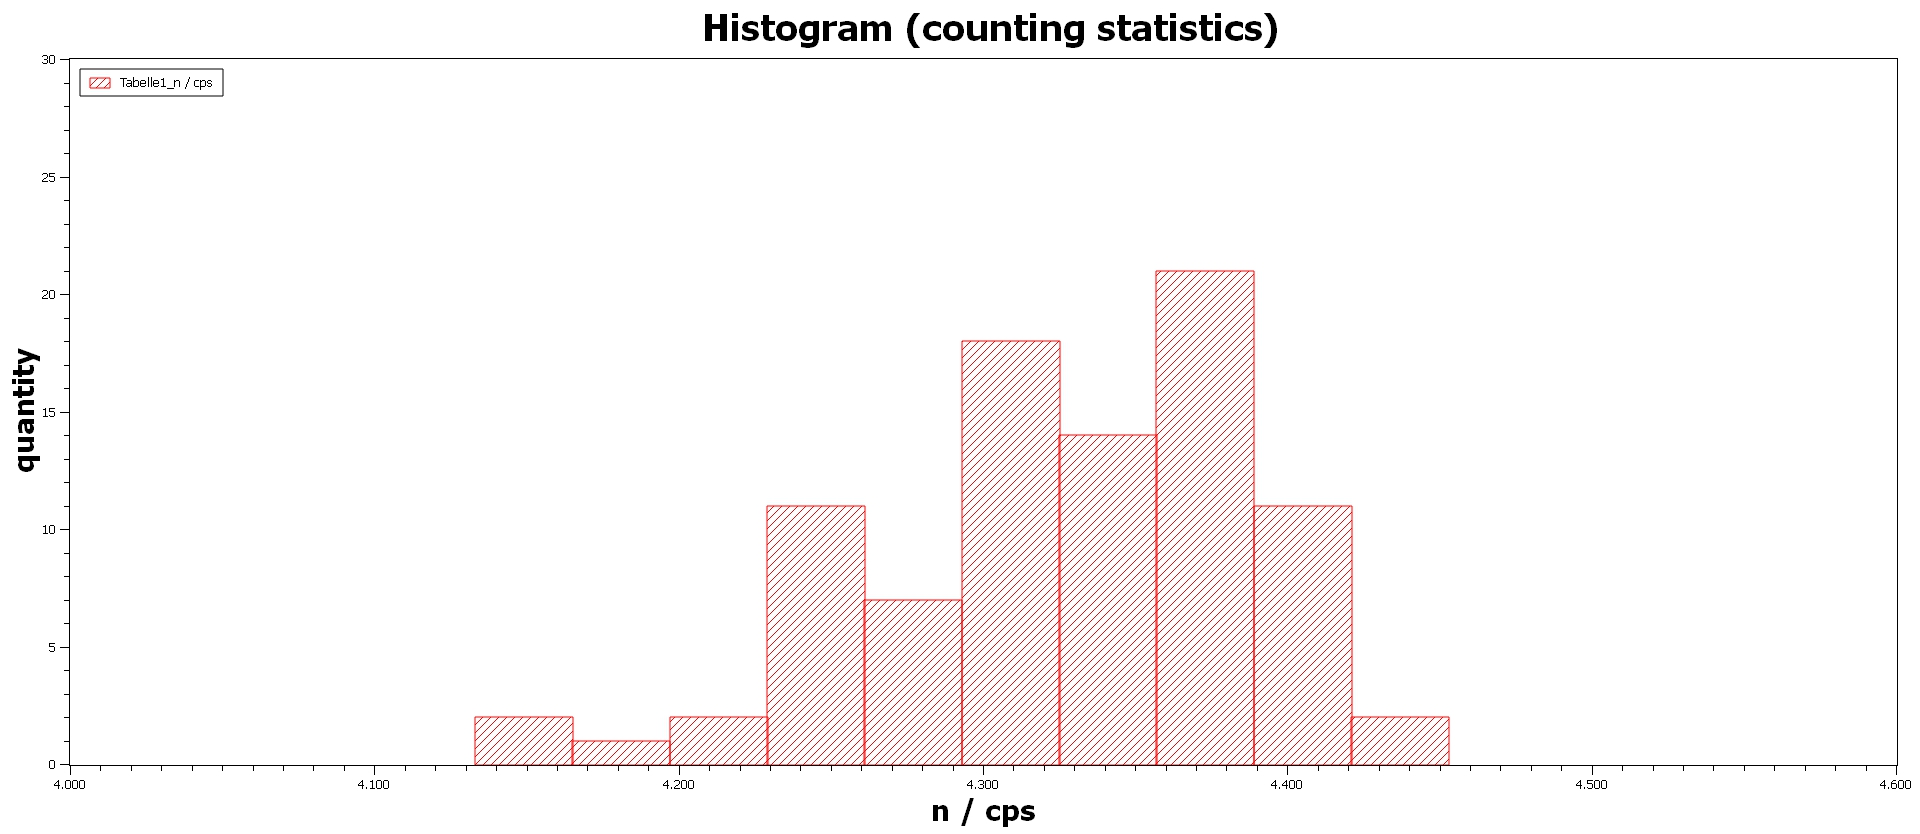
\includegraphics[width=.8\textwidth]{scidavis/Fig.9_Histogram (counting statistics).jpg}
 \caption[Histogram of the count rates]{Histogram of the count rates.}
 \label{fig:countStatsHistogram}
\end{figure}
With radioactive decay it cannot be said which atom will decay when. Since it is a statistical process, the histogram
can be described with a Poisson-distribution.
%
\section{Background Radiation}\label{sec:backgroundRadiation}
%
To investigate the background radiation the count rate was measured 90 times with no radiation source at a voltage of
\( U_{opt}=\SI{500}{V} \). The measurement stats are:
%
\begin{align}
\bar{n}     &=  \SI{3}{cps} \\
\sigma^{2}  &=  \SI{20}{(cps)^{2}} \\
\sigma      &=  \SI{4}{cps}
\end{align}
The measurement number was plotted versus the count rate:
\begin{figure}[H]
 \centering
 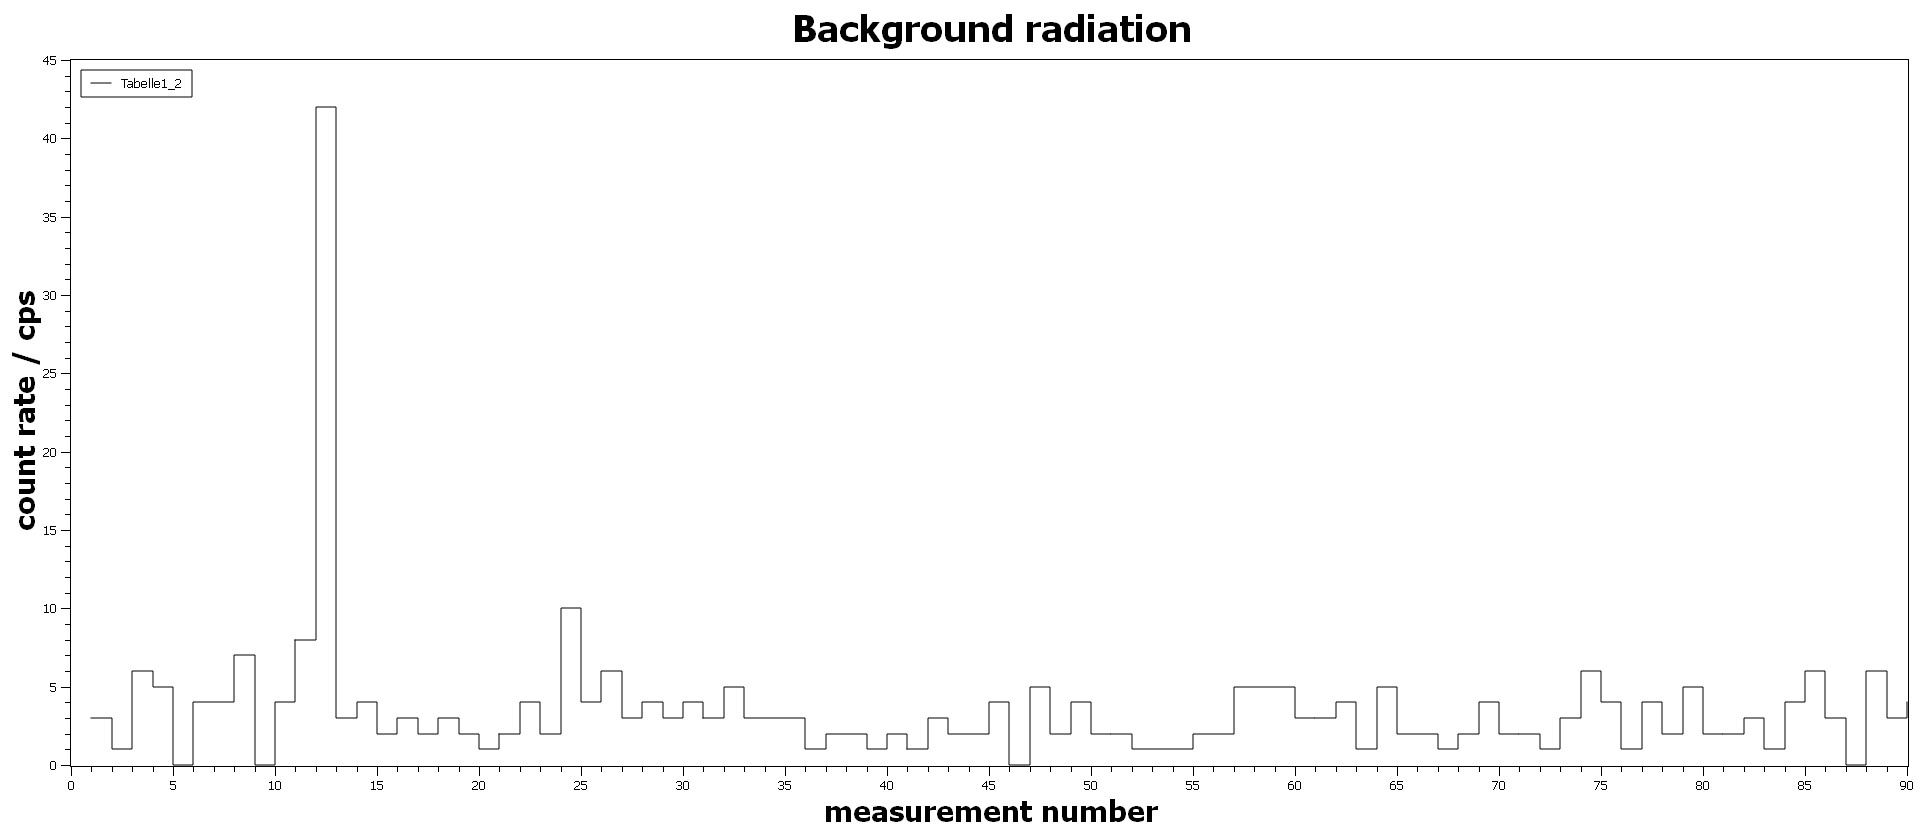
\includegraphics[width=.9\textwidth]{scidavis/Fig.10_Background radiation.jpg}
 \caption[Background radiation cps]{Measured counts caused by natural background radiation.}
 \label{fig:backgroundRad}
\end{figure}
With the associated distribution histogram:
\begin{figure}[H]
 \centering
 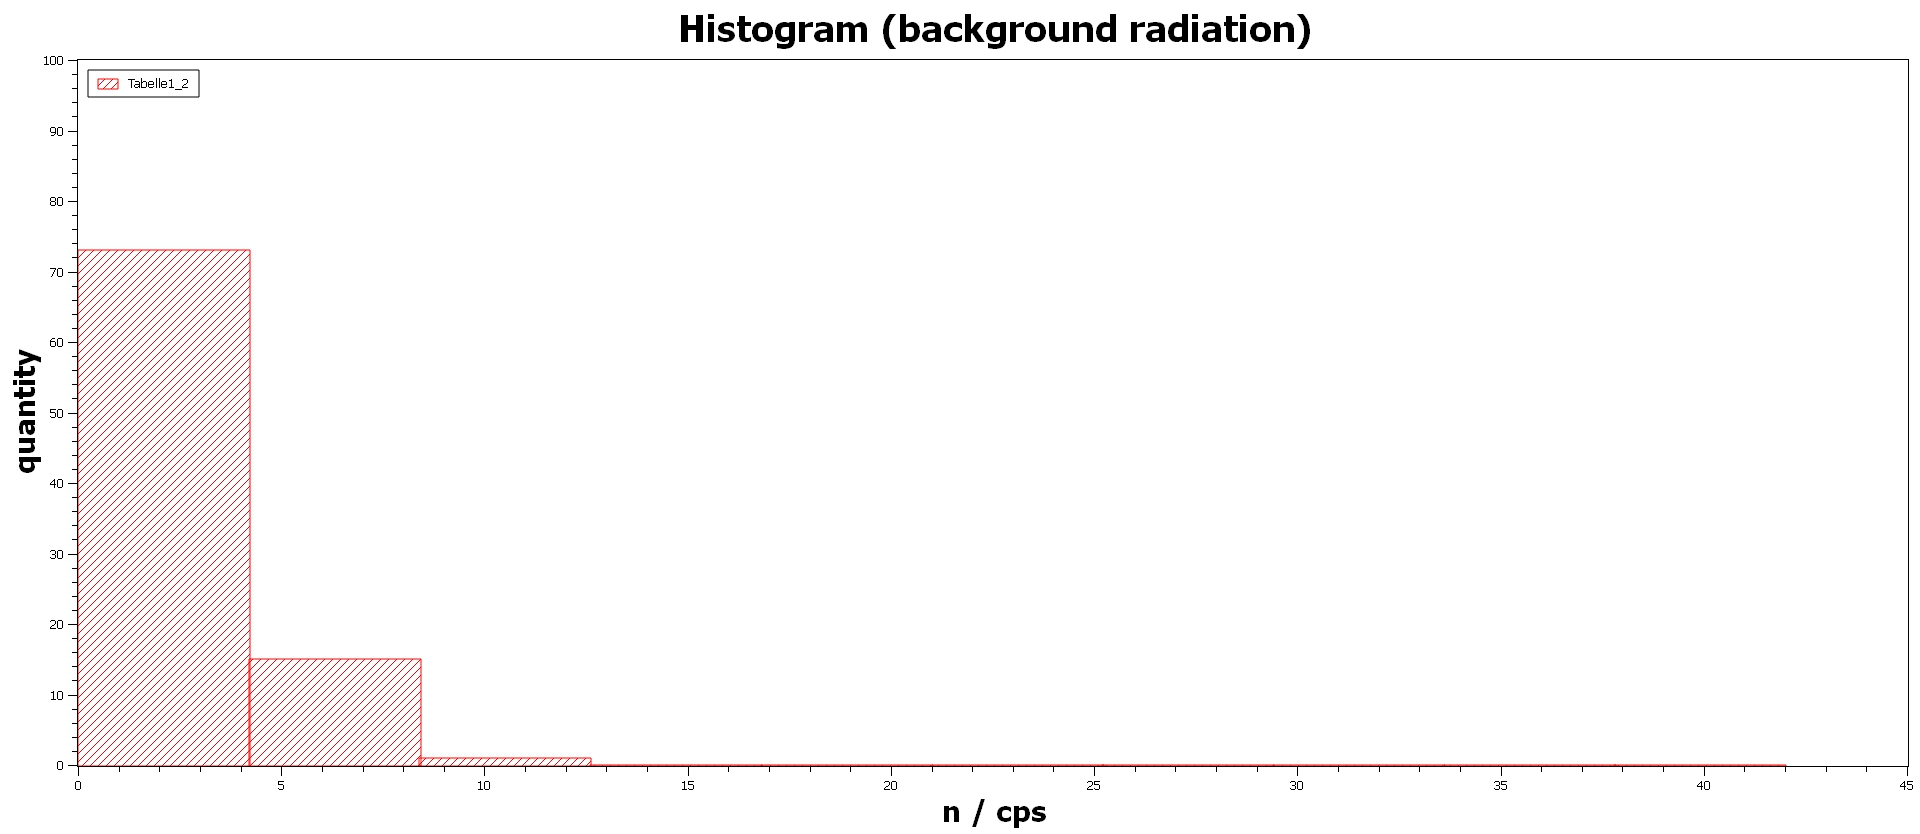
\includegraphics[width=.9\textwidth]{scidavis/Fig.11_Histogram (background radiation).jpg}
 \caption[Back Rad Hist]{Background Radiation Histogram.}
 \label{fig:backgroundRadHistogram}
\end{figure}
This histogram can also be described by a Poisson-distribution for the same reason as histogram of the counting
statistics.
%
\section{Natural Radioactivity}
%
Lastly, the radioactivity of Brazil Nuts was determined. The mean value of \( \bar{n}=\SI{3}{cps} \) indicates that the
radioactivity of the Brazil Nuts is very weak because it has the same mean value as the background radiation. However,
this does not have to mean that the Brazil Nuts do not emit any radiation. Because the tube was very close to the nuts,
the background radiation could not pass directly through the nuts, which implies that the rest of the radiation must have
come from the Brazil Nuts.
\begin{figure}[H]
 \centering
 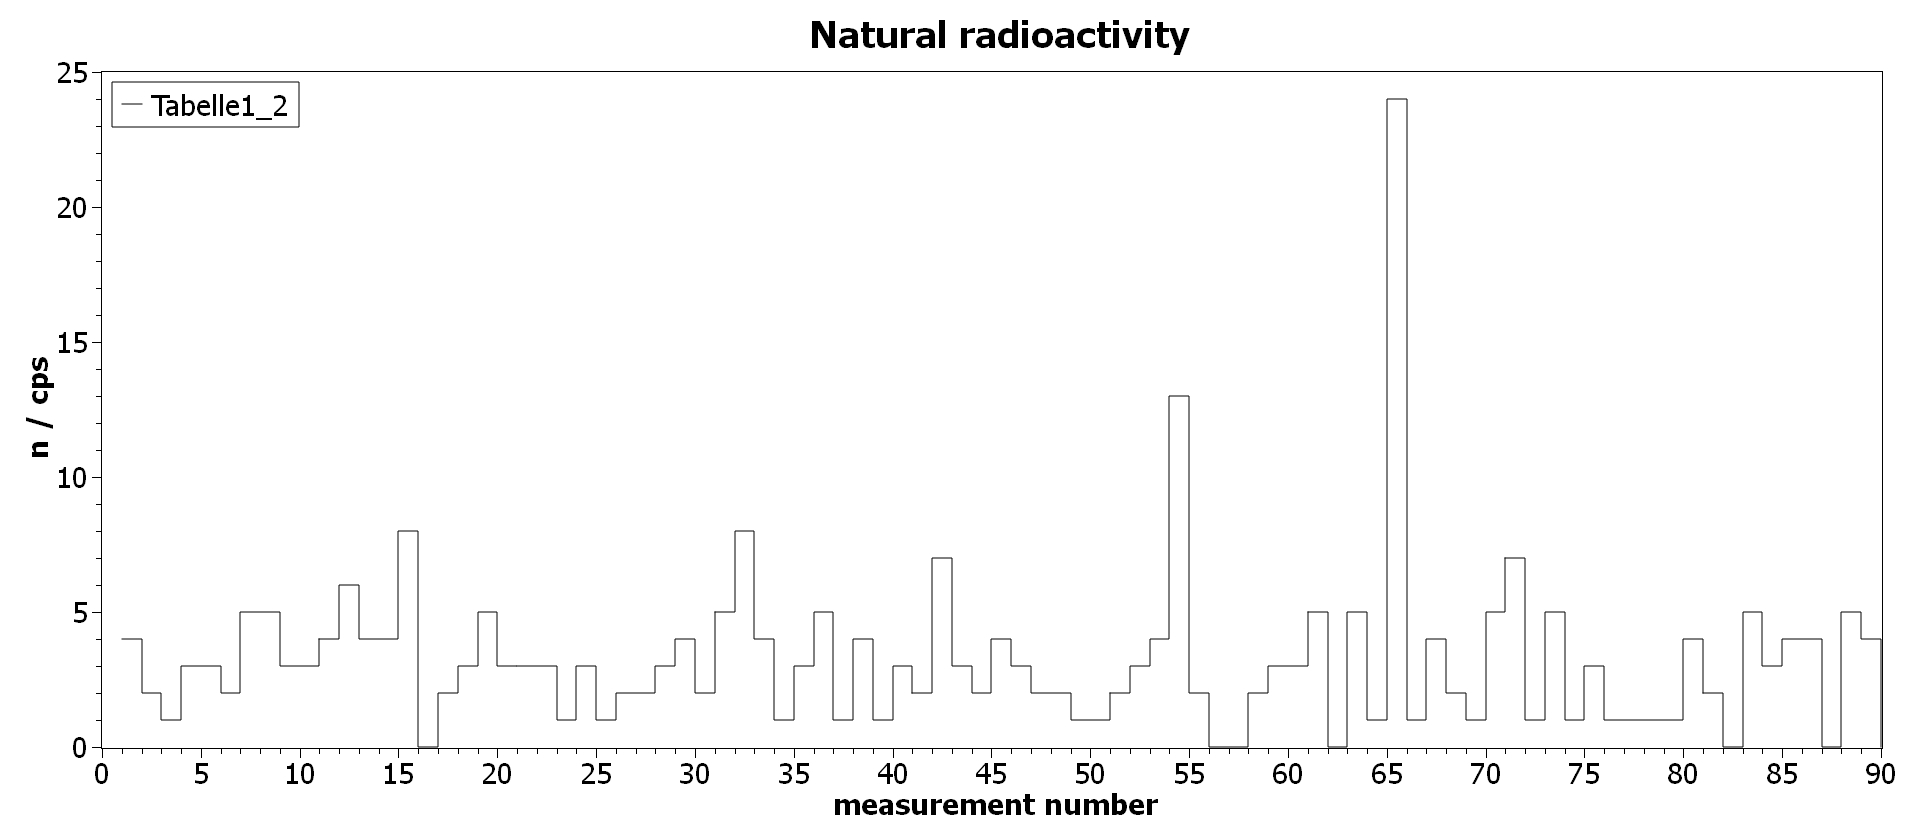
\includegraphics[width=.9\textwidth]{scidavis/Fig.12_Natural radioactivity.jpg}
 \caption[Brazil Nuts]{Radiation of Brazil Nuts.}
 \label{fig:brazilNutz}
\end{figure}
\chapter{Conclusion}
%
In a closing statement, the experiment is applicable to investigate the properties of a \textsc{Geiger-Mueller} tube and
clearly shows effects of radioactive decay. The oscilloscope shows the GMTs signal with its characteristic patterns
values as well as the recorded curves beeing very similar to the expected ones.\par
Unfortunately, the maximum adjustable voltage was only \( 600 V \). Therefore, the measurement ended somewhere in the
plateau area. The angular dependency of the count rate is plausible, as fewer particles arrive at an effective spatial
angle. The different absorption materials show that different material properties have a rather huge impact the rays passing
through. While some could drop the count rate to a degree comparable to the blank measurement discribed in \cref{sec:backgroundRadiation}
other seemingly had no impact at all. The raw measurement illustrates the statistical decay processes as well as the
functionality of the GMT.\par
Even though it was already common sense, measuring and visualizing the omnipresent background radiation as well as making
radioactivity of digestibles visible was a fascinating excercise. Plans are rising to give building a cloud chamber another
go.\par\medskip
While we assume it to be rather simple, yet we missed an introduction to the code used on the \micro-controller.
%-------------------
\newpage
\listoffigures 
\listoftables
\addchap{List of Symbols}
%
\begin{longtable}[l]{@{}ll@{}}%
	\( A \) & Area\\
	\( B \) & Magnetic flux density\\
	\( C \) & Capacitance\\
	\( C_{max} \) & Maximum capacitance\\
	\( D \) & Diameter\\
	\( D_{Ri} \) & Rod diameter\\
	\( D^* \) & Torsion constant\\
	\( I, I_c \) & Current of the eddy current brake\\
	\( J \) & Angular inertia\\
	\( J_S \) & Rotational inertia around the center\\
	\( J_P \) & Angular inertia of the pendulum\\
	\( J_R, J_{Ri} \) & Angular inertia of a cylindrical rod\\
	\( L, L_{Ri} \) & Rod length\\
	\( M \) & Torque\\
	\( \vec{M_{Frict}} \) & Frictional torque\\
	\( \vec{M_{Inert}} \) & Inertial torque\\
	\( \vec{M_{Rest}} \) & Restoring torque\\
	\( N \) & Number of turns\\
	\( R \) & Resistance\\
	\( T \) & Period time\\
	\( T_P \) & Period time of the pendulum without rod\\
	\( T_{P+Ri} \) & Period time of the pendulum with a rod\\
	\( U_0 \) & Initial voltage\\
	\( U_C \) & Capacitor voltage\\
	\( U_{ind} \) & Induced voltage\\
	\( U_{th} \) & Threshold voltage\\
	\\
	\( d \) & Plate distance\\
	\( k \) & Damping constant\\
	\( m, m_{Ri} \) & Rod mass\\
	\( n \) & Timer ticks\\
	\( o \) & Offset\\
	\( r \) & Distance to the rotational axis\\
	\( s \) & Sensitivity\\
	\( t \) & Time\\
	\( t_{th} \) & Time at threshold voltage\\
	\( x \) & Place\\
	\\
	\( \delta \) & Damping coefficient\\
	\( \delta_e \) & Exponential fit of \( \delta(I) \)\\
	\( \delta_p \) & Polynomial fit of \( \delta(I) \)\\
	\( \varepsilon_0 \) & Electric constant, vacuum permittivity\\
	\( \varepsilon_r \) & Relative permittivity\\
	\( \lambda \) & Differential equation coefficient\\
	\( \rho \) & Damping constant\\
	\(\tau\) & Time constant\\
	\( \varphi \) & Angle\\
	\( \hat{\varphi} \) & Angle amplitude\\
    \( \chi \) & Proportionality factor\\
    \( \chi' \) & Maximum resolution of the angular sensor\\
    \( \omega_0 \) & Angular frequency\\
    \( \omega_d \) & Natural angular frequency\\
    \(  \) & \\
\end{longtable}
\label{tab:glossar}
%
\addchap{List of Acronyms}
%
\begin{longtable}[l]{@{}ll@{}}%
    \( CC \) & Constant Current\\
    \( CCW \) & Counterclockwise\\
    \( COM-Port \) & Communication-Port\\
    \( CV \) & Constant Voltage\\
    \( CW \) & Clockwise\\
    \( GPIO \) & General Purpose Input / Output\\
    \( OS \) & Operating System\\
    \( PSU \) & Power Supply Unit\\
    \( USB \) & Universal Serial Bus\\
    \( \mu C \) & Microcontroller\\
\end{longtable}
\label{tab:acronyms}

\appendix
\chapter{Appendix}\label{sec:appendix}
%
\begin{figure}[H]%
    \centering
    \subfloat[$ I_{c}=\SI{0}{mA} $\label{subfig:damped-oscillation-0ma}]{\includegraphics[width=1\linewidth]{"messdaten/Damped Oscillation (0mA)"}}\\
    \subfloat[$ I_{c}=\SI{200}{mA} $\label{subfig:damped-oscillation-200ma}]{\includegraphics[width=1\linewidth]{"messdaten/Damped Oscillation (200mA)"}}
\end{figure}
\begin{figure}[H]\ContinuedFloat
    \subfloat[$ I_{c}=\SI{300}{mA} $\label{subfig:damped-oscillation-300ma}]{\includegraphics[width=1\linewidth]{"messdaten/Damped Oscillation (300mA)"}}\\
    \subfloat[$ I_{c}=\SI{400}{mA} $\label{subfig:damped-oscillation-400ma}]{\includegraphics[width=1\linewidth]{"messdaten/Damped Oscillation (400mA)"}}\\
    \subfloat[$ I_{c}=\SI{500}{mA} $\label{subfig:damped-oscillation-500ma}]{\includegraphics[width=1\linewidth]{"messdaten/Damped Oscillation (500mA)"}}%
    \caption[Course of tick rates at varying coil currents]{Plots of the tick rates over time with coil currents ranging from \SI{0}{mA} to \SI{500}{mA} in increments of \SI{100}{mA}}
    \label{fig:damped-oscillations}
\end{figure}
\printbibliography
%==========================================
\end{document}